% Copyright (c) 2009-2014 Ilya Palachev <iliyapalachev@gmail.com>

% Declare the class of document: size of paper, size of font, and etc.
% Type of the document is "article".
\documentclass[a4paper, 12pt, titlepage]{article} 

% Package that enables setting the size of free spaces at the border of the 
% page with the command  \geometry :
\usepackage{geometry}
\geometry {
   left=3cm,
   right=1.5cm,
   top=2cm,
   bottom=2cm
}

\usepackage[utf8]{inputenc}

\usepackage[english,russian]{babel}

\usepackage{amsmath}

%\usepackage{cmap}

\usepackage{indentfirst}

\usepackage{a4wide,amssymb}

%\usepackage[pdftex]{graphicx}

%\usepackage{wrapfig}

%\linespread{1.3}               % полтора интервала. Если 1.6, то два интервала
\pagestyle{plain}               % номерует страницы

\usepackage{graphicx}
\renewcommand{\topfraction}{1}
\renewcommand{\textfraction}{0}

% Package that enables usage of theorems and definition designed in a 
% standard way.
% http://en.wikibooks.org/wiki/LaTeX/Theorems
\usepackage{amsthm}

% Create environment for smart definitions
\theoremstyle{definition}
\newtheorem{SmartDefinition}{Определение}

% Create environment for smart theorems
\theoremstyle{plain}
\newtheorem{SmartTheorem}{Теорема}

% Create environment for smart lemmas
\theoremstyle{plain}
\newtheorem{SmartLemma}{Лемма}

% The following code enables back references:
\usepackage{color} 
\definecolor{darkgreen}{rgb}{0,.5,0} 
\usepackage[unicode,colorlinks,filecolor=blue,citecolor=darkgreen,pagebackref]
{hyperref}

% The package that provides symbols like \Square:
\usepackage{wasysym}

%opening
\title{Опорные методы восстановления выпуклых тел и их обобщения для задачи
восстановления многогранников по теневым и бликовым контурам \\ Технический
отчет}
\author{Палачев Илья}

\begin{document}

\maketitle

\tableofcontents

%%%%%%%%%%%%%%%%%%%%%%%%%%%%%%%%%%%%%%%%%%%%%%%%%%%%%%%%%%%%%%%%%%%%%%%%%%%%%%%%

\section{Введение}

\subsection{Исходная практическая проблема восстановления моделей алмазов по
теневым и бликовым контурам}

\subsection{Описание технологии построения моделей алмазов}

\subsection{Погрешности в теневых контурах и их последствия}

\subsection{Можно ли корректировать теневые контуры?}

\subsection{Смежные проблемы в компьютерной томографии, магнитно-резонансной
визуализации и обработке данных лазерного радара}

\subsection{Обзор работы}

%%%%%%%%%%%%%%%%%%%%%%%%%%%%%%%%%%%%%%%%%%%%%%%%%%%%%%%%%%%%%%%%%%%%%%%%%%%%%%%%

\newpage
\section{Основные понятия: преобразование двойственности и опорное представление
выпуклого тела}

Ключевыми понятиями, использующимися в данной работе для решения задачи
восстановления трехмерных тел являются понятие \textbf{преобразования
двойственности} и понятие \textbf{опорной функции выпуклого тела}. Первое из
них активно используется для решения задач вычислительной геометрии, поскольку
оно позволяет путем несложных преобразований над входными данными
переформулировать задачу так, чтобы понятия "точка" и "плоскость" поменялись
местами, что позволяет сводить новые задачи к таким, для которых уже имеются
известные методы решения. Примерами приложений преобразования двойственности
являются такие задачи как:

\begin{itemize}
 \item Нахождение пересечения многогранников.
 \item Нахождение треугольника минимальной площади с вершинами на заданном
множестве точек \cite{journals/BIT/ChazelleG1985}
 \item Разбиение множества точек на плоскости прямой на 2 класса, лежащих по
 разные стороны от прямой
\end{itemize}

и многие другие.

Второе понятие широко используется в такой области как \textbf{геометрическая
томография}. Суть подхода состоит в том, что любое выпуклое тело однозначно
определяется своей опорной функцией и задачу восстановления тела можно свести к
задаче восстановления опорной функции этого тела. В работе
\cite{journals/cviu/GhoshK98} производится анализ опорного представления и,
между прочим, исследуется его связь с преобразованием двойственности.

\newpage
\subsection{Понятие полярного преобразования двойственности}

Термин преобразования двойственности имеет хождение в вычислительной геометрии,
где он нашел широкое применение. В проективной геометрии данное понятие имеет
сходство с понятием поляры.

\begin{SmartDefinition}
 Пусть $\mathbb{R}^{n}$ - евклидово пространство. \textbf{Преобразованием 
двойственности} называется отображение $\delta$, определенное на множествах
аффинных подпространств пространства $R^{n}$, не содержащих начало координат
$0 = (0, \ldots, 0)$, и действующее следующим образом:
\begin{itemize}
 \item Пусть $A \neq 0$ -- подпространство размерности $0$ (т. е. точка),
 $A = (a_{1}, a_{2}, \ldots, a_{n}) \neq 0$. Тогда ему ставится в
 соответствие аффинное гиперпространство $\delta(A)$, описываемое линейным
 уравнением $a_{1} x_{1} + a_{2} x_{2} + \ldots + a_{n} x_{n} = 1$.
 \item Пусть $L$ -- некоторое аффиное гиперпространство (т. е. 
 подпространство размерности $n - 1$), не содержащее начало координат. Тогда его
 можно описать с помощью уравнения
 $a_{1} x_{1} + a_{2} x_{2} + \ldots + a_{n} x_{n} = 1$, причем коэффициенты
 этого уравнения определяются однозначно. Тогда преобразование двойственности
 ставит в соответствие $L$ точку $\delta(L) = (a_{1}, a_{2}, \ldots, a_{n})$.
 \item Пусть $L$ -- подпространство размерности $k \neq 0, n - 1, n$. Тогда ему
 ставится в соответствие подпространство размерности $n - k - 1$, определяемое
 как $\delta(L) = \{\delta(M) \; | \; L \subset M, dim M = n - 1\}$.
\end{itemize}

\end{SmartDefinition}

%% TODO: Добавить утверждение о том, что преобразование двойственности сохраняет
%% инцидентность

\newpage
\subsection{Пересечение многогранников и построение выпуклой оболочки --
двойственные задачи}

Свое распространение в вычислительной геометрии преобразование двойственности
получило благодаря статье Мюллера - Препараты \ref{Muller1978217}, в которой
описывается метод построения пересечения выпуклых многогранников. Он описан
также в классической монографии Препараты - Шеймоса "Введение в вычислительную
геометрию" \ref{Preparata:1985:CGI:4333}. Основная идея заключается в том, что
преобразование можно расширить на класс многогранных тел, если сопоставлять
вершинам -- грани, граням -- вершины, а всякому ребру, соединяющему некоторые
две точки $A_{1}$ и $A_{2}$, -- ребро, разделяющее грани $\delta(A_{1})$ и
$\delta(A_{2})$. Справедлива также следующая теорема:

%% TODO: Разъяснить понятия полиэдра, многогранника и многогранного множества.
%% Как они связаны между собой?

\begin{SmartTheorem}
 Если $P$ -- выпуклый полиэдр, содержащий начало координат, то таким же является
 и двойственный к нему полиэдр $P^{(\delta)}$.
\end{SmartTheorem}

Метод построения пересечения можно сформулировать в виде следующей теоремы:

\begin{SmartTheorem}
 Пусть $P$ и $Q$ -- полиэдры, имеющие общую точку. Предположим без ограничения
 общности, что эта точка -- начало координат. Тогда справедливо следующее
 соотношение:
 \begin{equation}
  \delta(P \bigcap Q) = conv (P^{(\delta)} \bigcup Q^{(\delta)})
 \end{equation}
\end{SmartTheorem}

Здесь через $conv (P^{(\delta)} \bigcup Q^{(\delta)})$ обозначена выпуклая
оболочка объединения многогранников $P^{(\delta)}$ и $Q^{(\delta)}$, которую
можно найти как выпуклую оболочку объединения множеств $V_{P}^{(\delta)}$ и
$V_{Q}^{(\delta)}$ вершин полиэдров $P^{(\delta)}$ и $Q^{(\delta)}$:

\begin{equation}
 conv (P^{(\delta)} \bigcup Q^{(\delta)}) = conv (V_{P}^{(\delta)} \bigcup
 V_{Q}^{(\delta)})
\end{equation}

Выпуклую оболочку точек можно построить с помощью известных алгоритмов
построения выпуклых оболочек, имеющих сложность $O(N \log N)$

Данный результат можно обобщить и на случай бесконечных выпуклых многогранных
множеств. В частности, справедлива следующая теорема:

\begin{SmartTheorem}
 Пусть $\pi_{1}, \pi_{2}, \ldots, \pi_{n}$ -- набор произвольных плоскостей в
 $\mathbb{R}^{3}$, а $R_{\pi_{1}}, R_{\pi_{2}}, \ldots, R_{\pi_{n}}$ --
 соответствующие им полупространства, содержащие начало координат $O$. Тогда
 пересечение этих полупространств можно найти с помощью следующего соотношения:
 \begin{equation}
  \delta \left(\bigcap \limits_{i = 1}^{n} R_{\pi_{i}} \right) =
  conv (\delta(\pi_{1}), \delta(\pi_{2}), \ldots, \delta(\pi_{n}))
 \end{equation}
\end{SmartTheorem}

\newpage
\subsection{Понятие опорной функции выпуклого тела}

Вторым ключевым понятием, которое будет использоваться в данной работе,
является так называемая \textbf{опорная функция выпуклого тела}, или 
\text{опорное представление выпуклого тела}.

Для простоты будем рассматривать выпуклые тела в трехмерном пространстве
$\mathbb{R}^{3}$, содержащие в своей внутренности начало координат $O$.
Для некоторых понятий будем давать определения и формулировки для случая
произвольной конечной размерности.

Как известно, выпуклое тело можно однозначно представить как пересечение 
полупространств всех его касательных плоскостей 
$K = \bigcap \limits_{x \in K} R_{x}$, где $R_{x}$ -- то из двух
полупространств, на которые плоскость $\pi_{x}$, касательная к телу $K$ в
точке $x$, делит $\mathbb{R}^{3}$, которое содержит в себе целиком все тело
$K$. Всякому выпуклому телу можно поставить в соответствие набор касательных 
плоскостей $\pi_{x}$, по которым его можно построить. Обратное неверно: не
всякому произвольному набору плоскостей можно поставить в соответствие тело,
касающееся всех этих плоскостей.

Всякую касательную плоскость $\pi_{x}$ можно однозначно охарактеризовать
единичным вектором нормали $u_{x}$ и расстоянием $h_{x}$ от начала координат 
$O$ до плоскости. Поскольку две разные касательные плоскости не могут иметь
одинаковые векторы нормалей, то можно рассматривать множество всех касательных
плоскостей выпуклого тела как функцию, определенную на всех единичных векторах
$u \in S_{2}$:

\begin{equation}h_{K}: S^{2} \to \mathbb{R}_{+}\end{equation}

Более общее понятие, включающее в себя выше указанное, было введено в 1903 году
Минковским.

\begin{SmartDefinition}
 \label{def:support-function}
 Будем называть \textbf{опорной функцией} выпуклого тела
 $K \subset \mathbb{R}^{n}$ следующую функцию
 $h_{K}: \mathbb{R}^{n} \to \mathbb{R}_{+}$:

 \begin{equation}h_{K}(u) = \max \limits_{x \in K}(x, u)\end{equation}
\end{SmartDefinition}

Если взять некоторую точку $u_{0}$ на единичной сфере $S^{n - 1}$, и вычислить
в ней значение опорной функции $h_{K}(u_{0})$, то по этим данным можно
построить касательную плоскость к выпуклому телу в некоторой (неизвестной!)
точке $x \in K$. Такую плоскость (в контексте, когда нет информации о положении
точки касания) принято называть опорной плоскостью.

\begin{SmartDefinition}
 \label{def:support-plane}
 \textbf{Опорной плоскостью} выпуклого тела $K$ по
 направлению $u \in S^{n - 1}$ называется плоскость с нормалью $u$, расстояние
 от которой до начала координат равно $h_{K}(u)$
\end{SmartDefinition}

Очевидно, что опорная функция выпуклого тела обладает следующим свойством:

\begin{equation}
 h_{K}(\lambda u) = \lambda h_{K}(u)
\end{equation}

Следовательно, для практики достаточно иметь дело только с ограничением опорной
функции на единичную сферу. В статье \cite{journals/jmiv/KarlKVW96} вводится
понятие \textbf{приведенной опорной функции}:

\begin{SmartDefinition}
 \label{def:support-plane}
 \textbf{Приведенной опорной функцией} выпуклого тела $K$ называется следующая
функция:
 \begin{equation}
 H_{K} (u) = h_{K} \left(\frac{u}{||u||}\right)
 \end{equation}
\end{SmartDefinition}

которая в действительности представляет собой расстояние от начала координат
$\mathbb{O}$ до опорной гиперплоскости по направлению $u$.

Более подробно свойства опорной функции рассматриваются в статье
\cite{journals/cviu/GhoshK98}.

\newpage
\subsection{Опорное и точечное зондирование -- двойственные задачи}

Еще одно применение преобразования двойственности было открыто в диссертации
Greschak \cite{thesis/Greschak1985}. В ней исследовались в частности две задачи
восстановления и была доказана их двойственность (т. е. сведение одной задачи к
другой с помощью преобразования двойственности и наоборот). Приведем здесь
коротко этот результат.

Определим так называемую \textbf{пробную функцию} некоторого выпуклого тела $K$:

\begin{equation}
 probe(x) = \alpha x, \;\;\; \alpha x \in \partial K
\end{equation}

В работе Greschak формулируются следующие две задачи:

\begin{flushleft}
 (\textbf{Задача 1}) Восстановить неизвестный ограниченный выпуклый
 многогранник $K$ путем выделения последовательности точек
 $x_{1}, x_{2}, \ldots, x_{k}$ и вычисления пробной функции $probe(x)$ тела $K$
 в каждой из этих точек.
\end{flushleft}

\begin{flushleft}
 (\textbf{Задача 2}) Восстановить неизвестный ограниченный выпуклый
 многогранник $K$ путем выделения последовательности плоскостей
 $r_{1}, r_{2}, \ldots, r_{k}$ и вычисления опорной функции $support(x)$ тела
 $K$ в каждой из этих плоскостей.
\end{flushleft}

При этом в диссертации опорная функция определяется на плоскостях, а не на
векторах, то есть $support(\pi) = \alpha \pi$, где $\alpha \pi$ -- плоскость,
опорная к телу $K$ (то есть такая, что $\alpha \pi \cap K \neq \varnothing$ и
тело $K$ целиком лежит по одну сторону от плоскости $\alpha \pi$).

В работе представлены результаты, представляющие собой решения задач (1) и 
(2). Одним из результатов диссертации Greschak является следующая теорема:

\begin{SmartTheorem}
 Если алгоритм $A$ восстанавливает неизвестный ограниченный выпуклый 
 многогранник $P$ в $\mathbb{R}^{n}$ путем выделения последовательности точек
 $x_{1}, x_{2}, \ldots, x_{k}$ и вычисления пробной функции $probe(x)$ в каждой 
 из этих точек, то существует также и двойственный алгоритм $A^{*}$, который
 восстанавливает двойственный многогранник $P^{*}$ многогранника $P$ путем
 выделения последовательности гиперплоскостей $r_{1}, r_{2}, \ldots, r_{k}$
 (который являются двойственными к точкам $x_{1}, x_{2}, \ldots, x_{k}$)
 и вычисления пробной функции $probe(x)$ в каждой из этих гиперплоскостей.
 Обратное также верно.
\end{SmartTheorem}



%%%%%%%%%%%%%%%%%%%%%%%%%%%%%%%%%%%%%%%%%%%%%%%%%%%%%%%%%%%%%%%%%%%%%%%%%%%%%%%%

\newpage
\section{Первичная и двойственная формулировка исходной проблемы}

Математическая формализация исследуемой задачи так или иначе должна быть
представлена как нахождение некоторого геометрического тела, которое бы
оптимальным образом соответствовало физическим измерениям, содержащим
погрешности. Любая формализация так или иначе должна представлять собой
математическую задачу, формулируемую в терминах точек, плоскостей, ребер,
многогранников и других геометрических объектов, решением которой будет являться
некоторый многогранник в $\mathbb{R}^{3}$.

Если взять эту формализацию, и заменить все слова "точка" на слова "плоскость",
а все слова "плоскость" на слова "точка", и так же поступить с со словами 
"содержит" и "содержится" (которые вообще можно заменить универсальным термином
"инцидентен / инцидентна"), то получится так называемая \textbf{двойственная
задача}.

Двойственная задача будет связана с исходной (которую будем называть
\textbf{первичной задачей}) следующим образом. Пусть $\mathfrak{F}$ --
входные данные первичной задачи (точки и плоскости в $\mathbb{R}^{3}$ с связи
между ними) и пусть $P$ -- многогранник, который является решением первичной
задачи для входных данных $\mathfrak{F}$. Тогда многогранник
$\delta(\mathfrak{P})$ будет являться решением двойственной задачи для входных
данных $\delta(\mathfrak{F})$.

Этот факт позволяет решать первичную задачу следующим образом:
\begin{itemize}
 \item Из первичных входных $\mathfrak{F}$ данных получить двойственные им 
данные $\delta(\mathfrak{F})$
 \item Найти решение двойственной задачи для входных данных
$\delta(\mathfrak{F})$. Пусть оно представляет собой некоторый многогранник $K$.
 \item По многограннику $K$ построить двойственный ему многогранник $P =
 \delta(\mathfrak{K})$ -- решений первичной задачи для входных данных\
 $\mathfrak{F}$.
\end{itemize}

Итак, задачу восстановления выпуклого тела по его теневым контурам можно
сформулировать двумя способами. Поясним вышесказанное и покажем, какие свойства
проблемы и какие подходы к ее решению можно вывести из этого соображения.

\newpage
\subsection{Первичная формулировка проблемы}

Первое, о чем следует сказать, есть то, что проблема возникает из прикладной
задачи, и поэтому допускает некоторую нечеткость в своей формулировке. Это дает
возможность предлагать различные математические формализации задачи.

\begin{SmartDefinition}
 Пусть $\pi$ -- некоторая плоскость в $\mathbb{R}^{3}$, проходящая через начало
 координат $O = (0, 0, 0)$. \textbf{Теневым контуром на плоскости $\pi$}
 называется всякая простая ломаная $C = A_{1} A_{2} \ldots A_{n}$ (т. е.
 ломаная без самопересечений) с конечным числом вершин, лежащая в плоскости
 $\pi$ таким образом, что ограниченная этой ломаной область в плоскости $\pi$
 содержит начало координат $O$.
\end{SmartDefinition}

\begin{SmartDefinition}
 Пусть $\nu = (\nu_{x}, \nu_{y}, \nu_{z}) \in \mathbb{R}^{3}$ -- некоторый
 вектор в $\mathbb{R}^{3}$ и пусть $\pi$ -- плоскость, задаваемая уравнением
 $\nu_{x} x + \nu_{y} y + \nu_{z} z = 0$, т. е. плоскость, проходящая через
 начало координат $O$ и имеющая нормаль $\nu$. \textbf{Теневым контуром по
 направлению $\nu$} называется всякий теневой контур на плоскости $\pi$.
\end{SmartDefinition}

\begin{SmartDefinition}
 Пусть $K$ - некоторое тело в $\mathbb{R}^{3}$ и пусть $\pi$ -- некоторая
 плоскость в $\mathbb{R}^{3}$. \textbf{Теневым контуром тела $K$ на плоскости
 $\pi$}, называется граница образа тела $K$ при отображении проецирования на
 плоскость $\pi$. Будем обозначать его через $C_{\pi}(K)$.
\end{SmartDefinition}

\begin{SmartDefinition}
 Пусть $K$ - некоторое тело в $\mathbb{R}^{3}$ и пусть $\nu = (\nu_{x},
 \nu_{y}, \nu_{z}) \in \mathbb{R}^{3}$ -- некоторый вектор в $\mathbb{R}^{3}$.
 \textbf{Теневым контуром тела $K$ по направлению  $nu$} называется теневой
 контур тела $K$ на плоскости $\pi$, задаваемой уравнением
 $\nu_{x} x + \nu_{y} y + \nu_{z} z = 0$, т. е. на плоскости, проходящей через
 начало координат $O$ и имеющей нормаль $\nu$. Будем обозначать его через
 $C_{\nu}(K)$
\end{SmartDefinition}

\begin{SmartDefinition}
 \textbf{Задачей восстановления трехмерного тела} называется конечный набор пар
 $\mathfrak{C} = \left\{(\nu_{i}, C_{i})\right\}_{i = 1}^{m}$, где $\nu_{1},
 \nu_{2}, \ldots, \nu_{m}$ -- некоторый набор векторов в $\mathbb{R}^{3}$,
 называемых векторами проецирования, и $C_{i}$ есть некоторый теневой контур 
 по направлению $\nu_{i}$ для каждого $i = 1, 2, \ldots, m$.
 Если все контуры $C_{i}$ являются выпуклыми многоугольниками, то задача
 $\mathfrak{C}$ называется \textbf{выпуклой}.
\end{SmartDefinition}

\begin{SmartDefinition}
 Задача восстановления трехмерного тела
 $\mathfrak{C} = \left\{(\nu_{i}, C_{i})\right\}_{i = 1}^{m}$ называется
 \textbf{тривиальной}, если существует такое трехмерное геометрическое тело $K$
 такое, что $C_{\nu_{i}}(K) = C_{i}$ для всех $i = 1, 2, \ldots, m$, т. е.
 теневым контуром тела $K$ по направлению $\nu_{i}$ является теневой контур
 $C_{i}$. Всякое такое геометрическое тело $K$, которое отвечает данным
 условиям, называется \textbf{решением тривиальной задачи восстановления}
 $\mathfrak{C}$
\end{SmartDefinition}

Ввиду того, что на практике входные данные являются измерениями теневых
контуров, выполненных с погрешностью, как правило все входные данные таковы,
что соответствующие им задачи восстановления не являются тривиальными. В данной
работе будет приведен критерий тривиальности задачи восстановления, который
удобно формулировать в терминах опорной функции. По сути одной из ключевых идей
данной работы является следующий подход к решению задач восстановления:

\begin{itemize}
 \item Тривиальные задачи восстановления решаются за линейное время
 \item Нетривиальные задачи можно сводить к \textit{близким} к ним тривиальным
 задачам.
\end{itemize}

Такой подход автоматически создает две проблемы:

\begin{itemize}
 \item Если нетривиальная задача имеет несколько решений, то какое из них
 следует предпочесть?
 \item Каким образом следует определить отношение близости между задачами
 восстановления, чтобы научиться сводить нетривиальные задачи к тривиальным?
\end{itemize}

Ответ на оба этих вопроса, а также их обоснование с точки зрения приложения,
будут рассмотрены в следующих разделах.

\begin{SmartDefinition}
 Пусть $\mathfrak{C} = \left\{(\nu_{i}, C_{i})\right\}_{i = 1}^{m}$ -- задача
 восстановления трехмерного тела. Набор теневых контуров
 $\{C_{1}, C_{2}, \ldots, C_{m}\}$ называется \textbf{согласованным}, если
 $\mathfrak{C}$ -- тривиальная задача восстановления, в противном случае он
 называется \textbf{несогласованным}.
\end{SmartDefinition}

\begin{SmartDefinition}
 Пусть $C$ -- теневой контур по направлению $\nu$. Он делит плоскость, в которой
 лежит, на две части: ограниченную, которую обозначим через $In C$ и
 неограниченную, которую обозначим $Out C$.
 \textbf{Теневым цилиндром, соответствующим теневому контуру} $C$, называется
 цилиндр
 \begin{equation}
  Cyl(C) = \{ x \in \mathbb{R}^{3}, x = y + t * \nu \; | \;
  y \in \overline{In C}, \; t \in \mathbb{R} \}
 \end{equation}
 где $\overline{In C}$ -- замыкание $In C$
\end{SmartDefinition}

Из приведенных выше определений непосредственно следует следующее утверждение:

\begin{SmartLemma}
 Пусть $\{C_{1}, C_{2}, \ldots, C_{m}\}$ -- некоторый набор теневых контуров.
 Для каждого $i = 1, 2, \ldots, m$ обозначим через
 $\pi_{i, j}, j = 1, 2, \ldots, m_{i}$ плоскости граней теневого цилиндра
 $Cyl(C_{i})$. При этом будем считать, что каждый цилиндр лежит по положительную
 сторону от всех своих плоскостей. Обозначим также через
 $l_{i, j} = \pi_{i, j} \cap \pi_{i, j + 1}$, т. е. прямые являющиеся ребрами
 теневого цилиндра $Cyl(C_{i})$.
 Набор теневых контуров $\{C_{1}, C_{2}, \ldots, C_{m}\}$ является согласованным
 тогда и только тогда, когда существует такой многогранник $K$, который для
 каждого $i = 1, 2, \ldots, m$ и $j = 1, 2, \ldots, m_{i}$ удовлетворяет
 следующим условиям:
 \begin{enumerate}
  \item $K$ лежит по положительную сторону от плоскости $\pi_{i, j}$
  \item Существует последовательность $A_{1} A_{2} \ldots A_{k}$ вершин
  многогранника $K$ такая, что для всех $s = 1, 2, \ldots, k - 1$ отрезок
  $A_{s} A_{s + 1}$ является ребром многогранника $K$, при этом все точки
  последовательности лежат в в плоскости $\pi_{i, j}$, а концевые точки 
  последовательности лежат на ребрах теневого цилиндра:
  $A_{1} \in l_{i, j - 1}$ и $A_{k} \in l_{i, j}$.
 \end{enumerate}
\end{SmartLemma}

%%%%%%%%%%%%%%%%%%%%%%%%%%%%%%%%%%%%%%%%%%%%%%%%%%%%%%%%%%%%%%%%%%%%%%%%%%%%%%%%

\newpage
\subsection{Двойственная формулировка проблемы}

Как уже было сказано, все утверждения предыдущих двух параграфов можно
переформулировать в терминах двойственности. В первую очередь интересен тот
факт, как при преобразовании двойственности изменяется утверждение
"трехмерное тело соответствует теневому контуру не плоскости". Ясность в
данный вопрос вносит следующее утверждение:

\begin{SmartLemma}
 Пусть $C$ -- теневой контур по направлению $\nu$, $Cyl(C)C$ -- соответствующий
 ему теневой цилиндр, а $\pi_{1}, \pi_{2}, \ldots, \pi_{m}$ -- плоскости граней
 соответствующего $Cyl(C)C$. Тогда образом теневого цилиндра $Cyl(C)$ при
 преобразовании двойственности $\delta$ является многоугольник $\delta(Cyl(C))$,
 лежащий в плоскости теневого контура $C$, т. е. в плоскости
 $\nu_{x} x + \nu_{y} y + \nu_{z} z = 0$, причем точки
 $\delta(\pi_{1}), \delta(\pi_{2}), \ldots, \delta(\pi_{m})$, являющиеся
 образами плоскостей $\pi_{1}, \pi_{2}, \ldots, \pi_{m}$ при преобразовании
 двойственности.
\end{SmartLemma}

Как нетрудно догадаться, в двойственном пространстве понятию теневого контура
будет соответствовать понятие плоского сечения. Поэтому задаче восстановления
объекта по теневым контурам будет соответствовать задача восстановления объекта
по его сечениям. Более строго эта идея в выпуклом случае выражается следующей
теоремой:

\begin{SmartTheorem}
 Пусть $\{C_{1}, C_{2}, \ldots, C_{m}\}$ -- некоторый набор \textbf{выпуклых}
 теневых контуров. Пусть
 $D_{1} = \partial \delta(Cyl(C_{1})),
  D_{2} = \partial \delta(Cyl(C_{21})),
  \ldots,
  D_{m} = \partial \delta(Cyl(C_{m}))$ -- границы многоугольников, являющихся
 образами теневых цилиндров при преобразовании двойственности.
 Тогда набор контуров $\{C_{1}, C_{2}, \ldots, C_{m}\}$ является набором теневых
 контуров некоторого \textbf{выпуклого} тела тогда и только тогда, когда
 существует выпуклое тело $K$ такое, что $D_{1}, D_{2}, \ldots, D_{m}$ будут
 являться его сечениями. При этом многогранник $P = \delta(K)$ будет
 представлять собой искомое тело.
\end{SmartTheorem}

%% TODO: Привести строгое формальное доказательство теоремы.

Данная теорема допускает обобщение на случай невыпуклых теневых контуров,
доказательство которого мы приведем в одной из последующих глав.

\begin{SmartTheorem}
 Пусть $\{C_{1}, C_{2}, \ldots, C_{m}\}$ -- некоторый набор теневых контуров
 (возможно, \textbf{невыпуклых}, но обязательно простых, т. к. в определение
 теневого контура входит условие простоты -- отсутствие самопересечений). Пусть
 $D_{1} = \partial \delta(Cyl(C_{1})),
  D_{2} = \partial \delta(Cyl(C_{21})),
  \ldots,
  D_{m} = \partial \delta(Cyl(C_{m}))$ -- границы многоугольников, являющихся
 образами теневых цилиндров при преобразовании двойственности (эти границы
 могут представлять из себя контуры, имеющие самопересечения).
 Тогда набор контуров $\{C_{1}, C_{2}, \ldots, C_{m}\}$ является согласованным
 тогда и только тогда, когда существует локально выпуклый многогранник $K$
 такой, что контуры $D_{1}, D_{2}, \ldots, D_{m}$ лежат на его границе и
 ребра этих контуров являются ребрами многогранника.
\end{SmartTheorem}

\newpage
\subsection{Обобщение для случая бликовых контуров}

Задача восстановления трехмерного тела по теневым проекциям имеет обобщение,
связанное с тем, что эмпирическим путем может быть получена дополнительная
информация о расположении граней -- это так называемые
\textit{бликовые контуры}. Они могут быть получены с помощью регистрации
отраженных бликов граней при отражении пучка света от поверхности кристалла.

В отличие от теневых контуров, бликовые контуры несут в себе информацию строго
о расположении только одной грани, причем заранее неизвестно какой грани.

Определения бликового контура трехмерного тела на плоскости, по направлению,
а также определение бликового цилиндра производятся очень похожим образом, как
для теневых контуров, за исключением того, что бликовые контуры не обязательно
должны содержать начало координат в ограничиваемой им области на плоскости.


\begin{SmartDefinition}
 Пусть $\pi$ -- некоторая плоскость в $\mathbb{R}^{3}$. \textbf{Бликовым
 контуром на плоскости $\pi$} называется всякая простая ломаная
 $C = A_{1} A_{2} \ldots A_{n}$ (т. е. ломаная без самопересечений) с конечным
 числом вершин, лежащая в плоскости $\pi$ таким образом, что ограниченная этой
 ломаной область в плоскости $\pi$ содержит начало координат $O$.
\end{SmartDefinition}

\begin{SmartDefinition}
 Пусть $\nu = (\nu_{x}, \nu_{y}, \nu_{z}) \in \mathbb{R}^{3}$ -- некоторый
 вектор в $\mathbb{R}^{3}$ и пусть $\pi$ -- плоскость, задаваемая уравнением
 $\nu_{x} x + \nu_{y} y + \nu_{z} z = 0$, т. е. плоскость, проходящая через
 начало координат $O$ и имеющая нормаль $\nu$. \textbf{Бликовым контуром по
 направлению $\nu$} называется всякий бликовый контур на плоскости $\pi$.
\end{SmartDefinition}

\begin{SmartDefinition}
 Пусть $K$ - некоторое тело в $\mathbb{R}^{3}$, пусть $f$ -- некоторая его
 грань и пусть $\pi$ -- некоторая плоскость в $\mathbb{R}^{3}$.
 \textbf{Бликовым контуром грани $f$ тела $K$ на плоскости $\pi$} называется
 граница образа грани $f$ при отображении проецирования на плоскость $\pi$.
 Будем обозначать его через $C_{\pi}(f)$.
\end{SmartDefinition}

\begin{SmartDefinition}
 Пусть $K$ - некоторое тело в $\mathbb{R}^{3}$, пусть $f$ -- некоторая его
 грань и пусть $\nu = (\nu_{x}, \nu_{y}, \nu_{z}) \in \mathbb{R}^{3}$ --
 некоторый вектор в $\mathbb{R}^{3}$.
 \textbf{Бликовым контуром грани $f$ тела $K$ по направлению  $nu$} называется
 бликовый контур тела $K$ на плоскости $\pi$, задаваемой уравнением
 $\nu_{x} x + \nu_{y} y + \nu_{z} z = 0$, т. е. на плоскости, проходящей через
 начало координат $O$ и имеющей нормаль $\nu$. Будем обозначать его через
 $C_{\nu}(f)$
\end{SmartDefinition}

Аналогичным образом определяется и задача восстановления трехмерного тела по
теневым и бликовым контурам -- как набор направлений и контуров, им
соответствующих.

Интересным представляется следующий вопрос: каким образом понятие бликового
контура формулируется в двойственном пространстве? Очевидно, что грань $f$
многогранника $P$ соответствует бликовому контуру $C$ тогда  и только тогда,
когда вершины грани $f$ лежат на ребрах бликового цилиндра $Cyl(C)$, то есть
на лежат на паре последовательных граней этого цилиндра. Поскольку в
двойственной постановке все точки перейдут в плоскости, а плоскости -- в точки,
грань $f$ и ее вершины $A_{1}, \ldots, A_{s}$ перейдут в вершину $\delta(f)$ и
грани $\delta(A_{1}), \ldots, \delta(A_{s})$, инцидентные этой вершине.
Бликовый цилиндр, как бесконечный объект, перейдет в многоугольник, лежащий в
плоскости, ортогональной образующим цилиндра и проходящей через начало координат
(это доказывается аналогично случаю теневого цилиндра), при этом грани бликового
цилиндра $\pi_{1}, \pi_{2}, \ldots, \pi_{s}$ перейдут в вершины этого
многоугольника $\delta(\pi_{1}), \delta(\pi_{2}), \ldots, \delta(\pi_{s})$.
Обозначим ребра $e_{1} = \delta(A_{1}) \cap \delta(A_{2}),
e_{2} = \delta(A_{2}) \cap \delta(A_{3}), \ldots,
e_{s} = \delta(A_{s}) \cap \delta(A_{1})$. Тогда условие соответствия грани $f$
многогранника $P$ бликовому контуру $C$ в двойственном пространстве
формулируется как условие того, что точки
$\delta(\pi_{1}), \delta(\pi_{2}), \ldots, \delta(\pi_{s})$ лежат на ребрах
$e_{1}, e_{2}, \ldots, e_{s}$ соответственно. Иными словами, двойственный образ
бликового контура многогранника всегда представляет собой некоторую часть
сечения двойственного многогранника.

\begin{figure}[ht]
 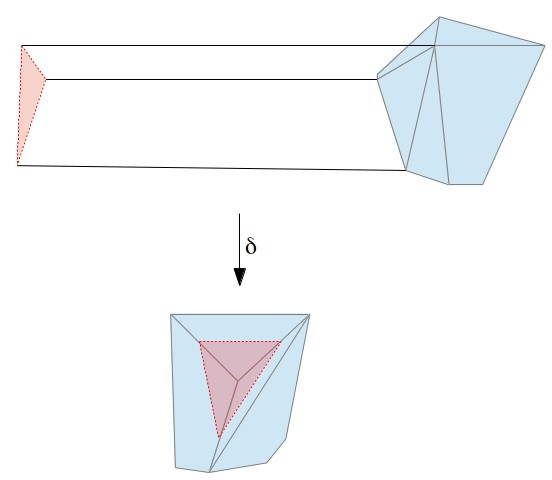
\includegraphics[width=10cm]{images/BlinkContourDual.jpg}
 \caption{Образ бликового контура при преобразовании двойственности.}
 \label{BlinkContourDual}
\end{figure}

Приведенный выше критерий можно проиллюстрировать с помощью рисунка
\ref{BlinkContourDual}. Заметим, что обозначенное на нижнем рисунке красным
цветом сечение не проходит ни через одну вершину двойственного многогранника.
Это связано с тем, что в противном случае одна из плоскостей граней исходного
многогранника обязана была бы быть плоскостью бликового цилиндра, что
невозможно.

В этом заключается принципиальное отличие бликовых и теневых контуров. Для
теневых контуров возможна такая их интерпретация, при которой
вершины двойственных образов теневых контуров являются вершинами двойственного
многогранника. Такая интерпретация возможна, если предположить, что каждый
теневой цилиндр составлен из плоскостей граней искомого многогранника.
Безусловно, такое предположение не реализуется в действительности, поскольку при
фотографировании одно и то же ребро появляется на нескольких кадрах сразу, и
почти наверное можно сказать, что ни на одном кадре нет скользящей проекции
ребра вдоль какой-нибудь инцидентной ему грани. Следуя
\cite{journals/pami/PrinceW90}, такую интерпретацию входных данных будем
называть \textbf{интерпретацией базового тела}.

\begin{figure}[ht]
 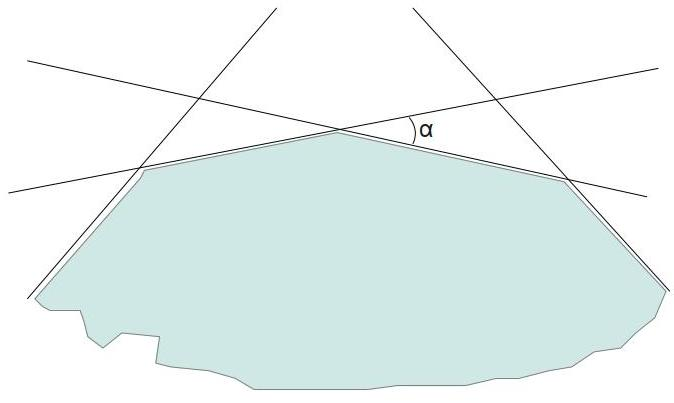
\includegraphics[width=10cm]{images/contour-1.jpg}
 \caption{Интерпретация базового тела}
 \label{contour-1}
\end{figure}

\begin{figure}[ht]
 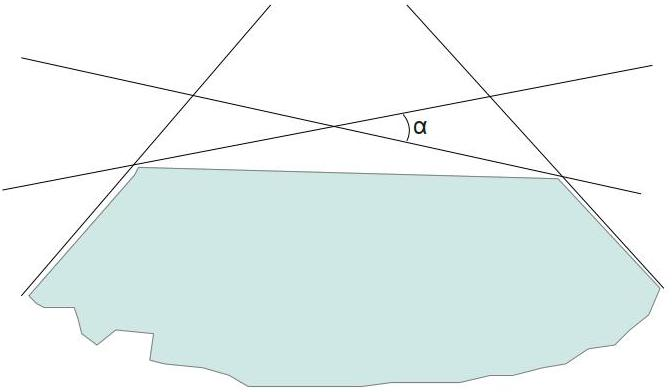
\includegraphics[width=10cm]{images/contour-2.jpg}
 \caption{Реальная конфигурация многогранника}
 \label{contour-2}
\end{figure}

Для наглядности на рисунках \ref{contour-1} и \ref{contour-2} показаны
интерпретация базового тела исходных входных данных и реальная конфигурация
многогранника, соответствующая таким входным данным.

Данная идея представляет из себя причину, по которой естественно возникает
потребность в разработке алгоритмов, учитывающих такую особенность входных
данных. Главная мотивация в этом деле -- снизить усложненность полученной
модели и попытаться приблизить ее к реальной конфигурации. Об этом будет
рассказано подробнее в последующих разделах.

Еще одно характерное отличие бликовых контуров от теневых -- это то, что они не
содержат начало координат в ограничиваемой ими конечной области плоскости. Это
существенным образом сказывается на свойствах образов этих контуров при
преобразовании двойственности. Для примера рассмотрим бликовый контур
$A_{1}A_{2}A_{3}A_{4}$, являющийся квадратом. изображенный на рисунке.
Введем на плоскости, в которой он лежит, двумерную систему координат $Oxy$.
Пусть вершины квадрата имеют координаты

\begin{align*}
& A_{1} = (1, 1), \\
& A_{2} = (3, 1), \\
& A_{3} = (3, -1), \\
& A_{4} = (1, -1) 
\end{align*}

тогда уравнения прямых, на которых лежат его стороны, представляют из себя
следующее:

\begin{align*}
& A_{1} A_{2}: \;\; y = 1 \\
& A_{2} A_{3}: \;\; \frac{1}{3} x = 1 \\
& A_{3} A_{4}: \;\; -y = 1 \\
& A_{4} A_{1}: \;\; x = 1
\end{align*}

При преобразовании двойственности вершины квадрата перейдут в следующие прямые:

\begin{align*}
& \delta(A_{1}) = \{ x + y = 1 \} \\
& \delta(A_{2}) = \{ 3 x + y = 1 \} \\
& \delta(A_{3}) = \{ 3 x - y = 1 \} \\
& \delta(A_{4}) = \{ x - y = 1 \}
\end{align*}

А прямые -- перейдут в следующие точки:

\begin{align*}
& \delta(A_{1} A_{2}) = (0, 1), \\
& \delta(A_{2} A_{3}) = (\frac{1}{3}, 0), \\
& \delta(A_{3} A_{4}) = (0, -1), \\
& \delta(A_{4} A_{1}) = (1, 0)
\end{align*}

Очевидно, что двойственный образ квадрата будет представлять из себя невыпуклый
четырехугольник (см. рис. \ref{BlinkSquareUnderDualTransform}).

\begin{figure}[ht]
 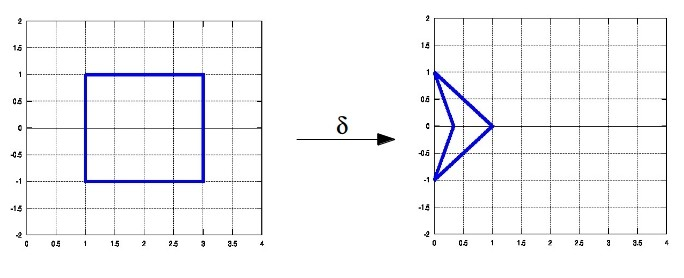
\includegraphics[width=10cm]{images/BlinkSquareUnderDualTransform.jpg}
 \caption{Бликовый контур, состоящий из квадрата и не содержащий начало
 координат, при преобразовании двойственности превращается в невыпуклый
 четырехугольник}
 \label{BlinkSquareUnderDualTransform}
\end{figure}


\newpage
\subsection{Образы одной вершины на разных контурах}

Очевидно, что одна и та же вершина при фотографировании камня может иметь образы
на нескольких снимках сразу. Вне всякого сомнения, это определенным образом
должно отразиться на свойствах полученных контуров. Такая ситуация
характеризуется тем, что несколько (более одного) ребер последовательных теневых
цилиндров пересекаются в одной точке (см. рис. \ref{OneVertexOnMultiplePhotos}).
Существуют методы, которые позволяют находить с помощью кластеризации подобные
вершины, и по ним восстанавливать трехмерные модели.

\begin{figure}[ht]
 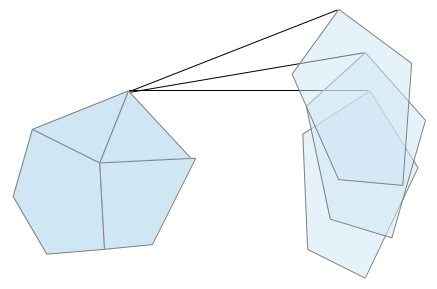
\includegraphics[width=10cm]{images/OneVertexOnMultiplePhotos.jpg}
 \caption{Образы одной вершины на разных контурах}
 \label{OneVertexOnMultiplePhotos}
\end{figure}

% TODO: Здесь нужно процитировать дипломную работу Степана. По всей видимости,
% он вводил определения и их здесь можно повторить...

В случае точных теневых контуров можно идентифицировать вершины разных контуров
как изображения одной и той же вершины исходного тела, если соответствующие
ребра теневых цилиндров пересекаются в одной точке. В реальном же случае,
когда все фотографии создаются с погрешностями, прямые могут и не пересечься.

Как можно идентифицировать изображения одной и той же вершины в двойственном
пространстве?

С точки зрения преобразования двойственности удобнее изучать этот вопрос в
терминах ребер. Пусть $e$ -- некоторое ребро исходного многогранника. Тогда для
тех кадров, на которых ребро $e$ видно, в соответствующих теневых цилиндрах
будет иметься по стороне, проходящей через $e$. Обозначим плоскости этих
сторон как $\pi_{1}, \pi_{2}, \ldots, \pi_{s}$. Все эти плоскости содержат в
себе (в реальном случае -- приближенно) ребро $e$:
$e \subset \pi_{i}, \;\; i = 1, 2, \ldots, s$. Поскольку преобразование
двойственности сохраняет отношение инцидентности между геометрическими
объектами, в двойственном пространстве полученные объекты будут снова
инцидентны друг другу. Образом ребра $e$ будет являться некоторый отрезок
$\delta(e)$, а образами плоскостей $\pi_{1}, \pi_{2}, \ldots, \pi_{s}$ --
точки $\delta(\pi_{1}), \delta(\pi_{2}), \ldots, \delta(\pi_{s}) \in e$,
содержащиеся во внутренности отрезка $e$.

Если же рассматривать некоторую вершину $v$, инцидентную ребрам
$e_{1}, \ldots, e_{k}$, то в двойственном пространстве она будет представлять
собой плоскость $\delta(v)$, содержащую в себе ребра
$\delta(e_{1}), \ldots, \delta(e_{k})$. Вершины-образы сторон теневых цилиндров
будут представлять собой точки, лежащие в одной плоскости, на сторонах одного
многоугольника.

Как изменятся выше приведенные суждения, если попытаться произвести их для
бликовых контуров? Всякая плоскость-сторона бликового цилиндра также проходит
через ребро $e$, изображением которого она является. Отличие от случая теневых 
контуров состоит в том, что стороны бликовых цилиндров не лежат между
плоскостями граней исходного многогранника, проходящих через это ребро. Для 
удобства можно ввести следующее определение:

\begin{SmartDefinition}
 Пусть $P$ -- многогранник в $\mathbb{R}^{3}$, $e$ -- некоторое ребро
многогранника $P$, а $f_{1}$ и $f_{2}$ -- содержащие его грани. Пусть $\pi_{1}$
и $\pi_{2}$ -- плоскости соответствующих граней. Тогда \textbf{углом теневой
видимости ребра} $e$ называется тот двугранный угол, образованный плоскостями
$\pi_{1}$ и $\pi_{2}$, который не содержит в себе внутренних точек
многогранника $P$ -- если такой двугранный угол существует.
\end{SmartDefinition}

В данных терминах можно сказать, что плоскости-стороны теневых цилиндров лежат
внутри углов теневой видимости соответствующих им ребер многогранника, а
плоскости-стороны бликовых цилиндров могут лежать, а могут и не лежать в этом
угле. В первом случае двойственные образы плоскостей-сторон будут являться
точками, лежащими на отрезке $e$, в последнем -- нет. Тем не менее, поскольку
$\alpha_{1}, \ldots, \alpha_{l}$ (бликовые плоскости-стороны) проходят через
обе точки $A_{1}$ и $A_{2}$ (вершины ребра $e$), их двойственные образы -- точки
$\delta(\alpha_{1}), \ldots, \delta(\alpha_{l})$ лежат в плоскостях
$\delta(A_{1})$ и $\delta(A_{2})$, то есть лежат на прямой, являющейся
пересечением этих плоскостей. Обозначим эту прямую через $l$. Верно утверждение,
что $\delta(\pi_{1}) \in l$ и $\delta(\pi_{2})$, где $\pi_{1}$ и $\pi_{2}$ --
стороны угла теневой видимости, т. е. плоскости граней многогранника $P$,
содержащие ребро $e$. Двойственные образы плоскостей-сторон теневых цилиндров
будут лежать на прямой $l$ между точками $\delta(\pi_{1})$ и $\delta(\pi_{2})$,
а плоскости-стороны бликовых цилиндров будут лежать на прямой $l$ вне отрезка
$\delta(e) = \delta(\pi_{1}) \delta(\pi_{2})$.

По какую сторону от отрезка $\delta(e)$ будет лежать двойственный образ той или 
иной бликовой плоскости-стороны? Рассмотрим такую бликовую плоскость-сторону 
$\pi_{0}$, которая помимо того, что проходит через отрезок $e$, содержит также 
в себе начало координат $O$ (т. е. рассмотрим плоскость $O A_{1} A_{2}$). 
Поскольку свободный член уравнения, описывающее плоскость $O A_{1} A_{2}$
равен $0$, то преобразование двойственности на нем не определено. Все бликовые 
плоскости-стороны, проходящие через ребро $e$, лежат либо по одну, либо по 
другую сторону от плоскости $O A_{1} A_{2}$. В зависимости от того, по какую 
сторону они лежат, точки, являющиеся их двойственными образами, будут лежать
по ту или по другую сторону от ребра $\delta(e)$ на прямой $l$ (см. рис.
\ref{DualShadowBlinkSides}).

\begin{figure}[ht]
 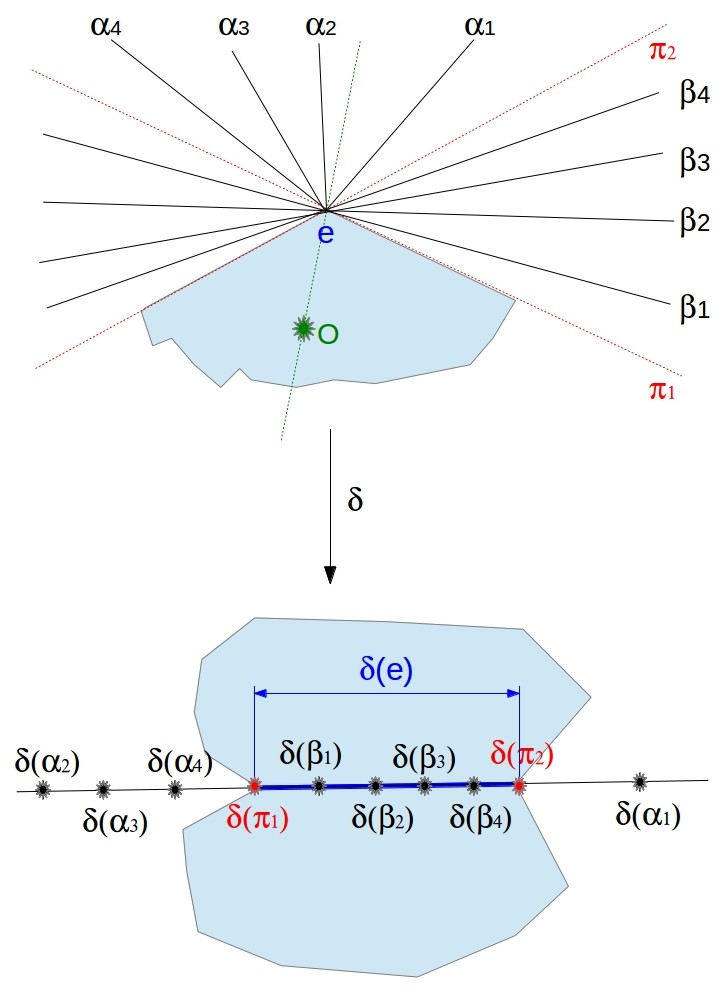
\includegraphics[width=10cm]{images/DualShadowBlinkSides.jpg}
 \caption{Двойственные образы плоскостей-сторон теневых и бликовых цилиндров}
 \label{DualShadowBlinkSides}
\end{figure}

\newpage
\subsection{Разрешение нарушений плоскостности при подвижке вершины}

Отступим немного от принятой задачи восстановления и предположим, что уже
построено некоторое трехмерное тело. Допустим, что с целью устранения дефекта в
модели требуется подвинуть некоторую вершину из одного положения в другое.
Можно ли каким-то образом воспользоваться свойствами преобразования
двойственности, чтобы решить эту задачу?

Для простоты предположим, что построенный многогранник -- выпуклый. Для начала
рассмотрим задачу на простом примере. Пусть
$P = A_{0} A_{1} A_{2} A_{3} A_{4} A_{5} A_{6} A_{7}$ -- куб со
стороной длины $2$, координаты вершин которого имеют величины $-1$ и $1$. Его
вершины имеют следующие координаты:

\begin{align*}
 & A_{0} = (-1, -1, -1) \\ & A_{1} = (1, -1, -1) \\
 & A_{2} = (1, 1, -1)   \\ & A_{3} = (-1, 1, -1) \\
 & A_{4} = (-1, -1, 1)  \\ & A_{5} = (1, -1, 1)  \\
 & A_{6} = (1, 1, 1)    \\ & A_{7} = (-1, 1, 1)
\end{align*}

Уравнения плоскостей его граней имеют следующий вид:

\begin{align*}
 & A_{0} A_{1} A_{2} A_{3} : z = -1 \Leftrightarrow -z = 1 \\
 & A_{4} A_{5} A_{6} A_{7} : z = 1 \\
 & A_{0} A_{1} A_{5} A_{4} : y = -1 \Leftrightarrow -y = 1 \\
 & A_{1} A_{2} A_{6} A_{5} : x = 1 \\
 & A_{2} A_{3} A_{7} A_{6} : y = 1 \\
 & A_{3} A_{0} A_{4} A_{7} : x = -1 \Leftrightarrow -x = 1 \\
\end{align*}

% TODO: Добавить сюда изображение куба P.

Двойственные образы вершин куба представляют из себя плоскости, имеющие
следующие уравнения:

\begin{align*}
 & \delta(A_{0}) = \{ -x - y - z = 1 \} \\
 & \delta(A_{1}) = \{  x - y - z = 1 \} \\
 & \delta(A_{2}) = \{  x + y - z = 1 \} \\
 & \delta(A_{3}) = \{ -x + y - z = 1 \} \\
 & \delta(A_{4}) = \{ -x - y + z = 1 \} \\
 & \delta(A_{5}) = \{  x - y + z = 1 \} \\
 & \delta(A_{6}) = \{  x + y + z = 1 \} \\
 & \delta(A_{7}) = \{ -x + y + z = 1 \}
\end{align*}

Двойственные образы граней куба представляют из себя следующие точки:

\begin{align*}
 & \delta(A_{0} A_{1} A_{2} A_{3}) = ( 0,  0, -1) \\
 & \delta(A_{4} A_{5} A_{6} A_{7}) = ( 0,  0,  1) \\
 & \delta(A_{0} A_{1} A_{5} A_{4}) = ( 0, -1,  0) \\
 & \delta(A_{1} A_{2} A_{6} A_{5}) = ( 1,  0,  0) \\
 & \delta(A_{2} A_{3} A_{7} A_{6}) = ( 0,  1,  0) \\
 & \delta(A_{3} A_{0} A_{4} A_{7}) = (-1,  0,  0)
\end{align*}

Следовательно, двойственным образом куба $P$ является октаэдр $\delta(P)$ с
вершинами в концах единичных отрезков на осях координат $Ox$, $Oy$ и $Oz$.

% TODO: Добавить сюда изображение октаэдра \delta(P).

Пусть требуется подвинуть точку $A_{6} = (1, 1, 1)$ в некоторое новое положение
$A_{6}^{*} = (1 + d_{1}, 1 + d_{2}, 1 + d_{3})$.

\textbf{1. } Рассмотрим сначала случай $d_{1} > 0, d_{2}, d_{3} > 0$.

Если оставить все остальные вершины и грани куба без изменения, то трех гранях,
содержащих вершину $A_{6}$, т. е. в гранях
$A_{1} A_{2} A_{6} A_{5}, A_{2} A_{3} A_{7} A_{6}, A_{4} A_{5} A_{6} A_{7}$,
нарушится плоскостность, поскольку вершины этих граней теперь не будут лежать в
одной плоскости. Как эта ситуация выглядит в двойственном пространстве?

Очевидно, что всякое перемещение точки, удаляющее ее от начала координат,
соответствует перемещению ее двойственного образа, приближающему его к началу
координат в двойственном пространстве. В данном случае двойственный образ
вершины $A_{6}$ после перемещения будет представлять из себя следующее:

\begin{equation*}
 \delta(A_{6}^{*}) = \{ (1 + d_{1}) x + (1 + d_{2}) y + (1 + d_{3}) z = 1 \}
\end{equation*}

Новая плоскость по прежнему пересекает грани, смежные с ней по общему ребру, по
некоторому ребру, а грани, смежные с ней по вершине -- теперь пересекает по
некоторому новому образовавшемуся ребру (см. рис. ).

%%%%%%%%%%%%%%%%%%%%%%%%%%%%%%%%%%%%%%%%%%%%%%%%%%%%%%%%%%%%%%%%%%%%%%%%%%%%%%%%

\newpage
\section{Опорные методы и опорные задачи восстановления выпуклых
тел (исторический обзор)}

В предыдущем разделе мы пытались рассматривать различные интерпретации входных
данных задачи восстановления трехмерного тела, назвали эти данные
\textit{задачами восстановления}. Однако строгого понятия \textit{решения
задачи восстановления} дано не было. В первую очередь это обусловлено самой
сущностью прикладной задачи, в которой строгого понимания, какой именно объект
в конечном счете нужно получить, -- нет. На практике требуется получить
тело, которое бы наилучшим образом приближало исходное (с точки зрения
близости в евклидовой метрике между вершинами, ребрами и гранями исходного и
восстановленного многогранников), -- с одной стороны, а с другой -- которое бы
повторяло основные топологические особенности тела.

Оказывается, существуют такие ситуации, когда эти две цели не могут быть
удовлетворены одновременно. На практике часто возникают ситуации, когда
построенная модель близко расположена к требуемым позициям в пространстве,
однако вместо одной крупной грани в ней присутствуют несколько более
мелких, или когда вместо одной вершины с большим числом инцидентных ей
ребер (т. е. высокой степени), однако в модели вместо одной вершины присутствуют
несколько близко расположенных вершин меньшей степени.

Любая математическая формализация задачи приводит к упрощению, если мы
формулируем задачи, которые можно эффективно решить с помощью существующих
вычислительных методов. Поэтому целесообразным выглядит подход, когда
предлагается \textit{несколько вариантов решения}, а пользователь программного
пакета имеет возможность выбирать среди них, а еще лучше -- "усреднять"
различные решения между собой, чтобы получить такое, которое бы
было бы удовлетворительно с точки зрения сразу нескольких критериев качества
модели.

В результате обзора некоторого количества статей из математических и
физических журналов по геометрической томографии, мат. статистике и компьютерной
геометрии было замечено сходство изучаемой задачи с теми, которые
рассматриваются в тех статьях. А именно, было замечено, что входные данные
задачи восстановления моделей алмазов можно переформулировать в терминах входных
данных некоторых задач геометрической томографии. Поскольку в этой смежной
области уже был накоплен заметный опыт решения подобных задач, мы попытались
перенять его, и чтобы это сделать, а также понять, насколько ценными будут
полученные алгоритмы, мы постарались ответить на следующие вопросы:

\begin{enumerate}
 \item Какие формализации задачи восстановления геометрических тел существуют в
геометрической томографии?
 \item Какие решения поставленных задач могут быть построены с помощью
разработанных методов?
 \item Каким образом можно интерпретировать нашу исходную задачу восстановления
тела по теневым (а также бликовым) контурам как задачу, которую можно решить с
помощью разработанных методов?
 \item Какую практическую ценность будут иметь полученные результаты?
 \item Можно ли модифицировать разработанные методы таким образом, чтобы
повысить ценность этих результатов?
\end{enumerate}

Если смотреть с точки зрения этого плана, то в предыдущем разделе мы несколько
забежали вперед, -- а именно, уже введен основной геометрический аппарат этих
статей, и на его основе произведено несколько попыток интерпретации исходной
задачи. В настоящем разделе мы постараемся осветить первые два пункта плана, а
в следующем -- приведем идею, позволяющую оптимизировать имеющиеся алгоритмы с
точки зрения быстродействия, а в еще одном разделе -- ответим на третий вопрос.

\newpage
\subsection{Задача двумерного восстановления выпуклого тела по равномерно
распределенным измерениям опорной функции}

\subsubsection{Прикладная задача из компьютерной томографии}

В работе \cite[Prince - Willsky (1990)]{journals/pami/PrinceW90}
рассматриваются алгоритмы для восстановления \textbf{двумерных} выпуклых тел по
измерениям их опорных функций. Изначально изучение данной проблемы было
мотивировано задачей из компьютерной томографии. А именно, в томографии
делаются измерения интегралов плотности поглощения излучения объектом вдоль
различных фиксированных прямых. Допустим, что известны интегралы плотности
поглощения по пучку прямых $L(t, \theta)$, где угол $\theta$ фиксирован. Тогда
по этой информации можно определить положение двух опорных прямых к данному
объекту (см. рис. \ref{tomography-application}).

\begin{figure}[ht]
    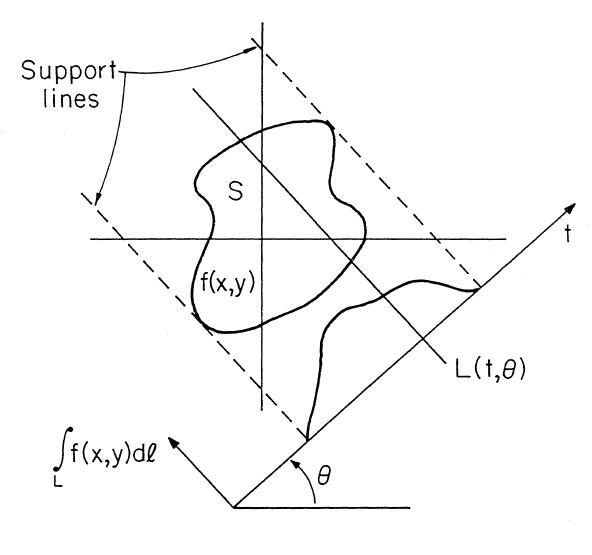
\includegraphics[width=10cm]{images/tomography-application.jpg}
    \caption{Граница носителя функции плотности поглощения определяет две
    опорные прямые к объекту}
    \label{tomography-application}
\end{figure}

По имеющимся измерениям опорной функции можно построить грубое приближение
рассматриваемого тела -- путем обыкновенного пересечения полуплоскостей,
соответствующих опорным прямым. Однако на практике измерения подвержены
ошибкам и известны лишь с некоторой точностью. Так, может оказаться, что
после пересечения построенное тело будет касаться не всех заданных прямых.
Это приводит к тому, что всего одно грубое измерение может заблокировать
воздействие других (более точных) измерений на результат (см. рис.
\ref{inconsistent}).

\begin{figure}[ht]
    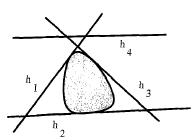
\includegraphics[width=10cm]{images/inconsistent-support-planes.jpg}
    \caption{В случае неточных измерений опорной функции тело нельзя строить
    как пересечение полупространств}
    \label{inconsistent}
\end{figure}

Prince и Willsky рассматривают в своей статье случай, когда измерения опорной
функции получаются по фиксированному набору направлений

\subsubsection{Критерий согласованности набора опорных чисел (в двумерном
случае и при равномерном распределении направлений измерения)}

Ключевым понятием в статье является следующее

\begin{SmartDefinition}
 \label{def:support-vector}
 \textbf{Набором опорных чисел}
 $(h_{0}, h_{1}, \ldots, h_{M - 1})^{T}$выпуклого тела $K$ по заданному набору
 направлений $u_{i}, i = 0, \ldots, M - 1$ называется называется вектор в
 $\mathbb{R}^{M}$, составленный из значений опорной функции по соответствующим
 направлениям: $(h_{K}(u_{0}), h_{K}(u_{1}), \ldots, h_{K}(u_{M - 1}))^{T}$.
\end{SmartDefinition}

Вектор, составленный из набора опорных чисел, является по сути аналогом
непрерывной опорной функции. Если говорить более точно, опорный вектор есть
сеточная функция, соответствующая непрерывной функции $h(\theta)$. Всякая ли
непрерывная функция является опорной функцией некоторого выпуклого тела? Ответ
на этот вопрос дает следующая теорема:

\begin{SmartTheorem}
 \label{thm:support-function-criterion}
 \textbf{Критерий опорной функции}.

 Непрерывная функция $h : \mathbb{R} \to \mathbb{R}_{+}$ является опорной
 функцией некоторого выпуклого тела тогда и только тогда, когда для всех
 $\theta \in \mathbb{R}$ выполнено следующее неравенство:

 \begin{equation}
 h''(\theta) + h(\theta) \geq 0
 \end{equation}
\end{SmartTheorem}


Основным теоретическим результатом статьи, на котором основаны все алгоритмы,
является следующая

\begin{SmartTheorem}
 \label{thm:support-vector-criterion}
 \textbf{Опорная теорема}

 Набор действительных чисел $h \in \mathbb{R}^{M}, M \leq 5$ является набором
 опорных чисел тогда и только тогда, когда

 \begin{equation}
  h^{T} C \leq (0, \ldots, 0)
 \end{equation}

 где $C$ -- $M \times M$ матрица, заданная следующим образом:

 \begin{equation}
  C =
  \left(
  \begin{array}{ccccccc}
       1 &     -k &      0 & \ldots &      0 &      0 &     -k \\
      -k &      1 &     -k & \ldots &      0 &      0 &      0 \\
       0 &     -k &      1 & \ldots &      0 &      0 &      0 \\
  \vdots & \vdots & \vdots & \ddots & \vdots & \vdots & \vdots \\
       0 &      0 &      0 & \ldots &      1 &     -k &      0 \\
       0 &      0 &      0 & \ldots &     -k &      1 &     -k \\
      -k &      0 &      0 & \ldots &      0 &     -k &      1 \\
  \end{array}
  \right)
 \end{equation}

 где $k = 1 / (2 cos(\frac{2 \pi}{M}))$.
\end{SmartTheorem}

Важно также заметить сходство между условием для непрерывной опорной функции и
условием для дискретного вектора, составленного из набора опорных чисел.
Величина $ - h^{T} C$, компоненты которой должны быть неотрицательными, является
по сути дискретным аналогом величины $h''(\theta) + h(\theta)$. Расширяя эту
аналогию, авторы статьи приводят геометрическую интерпретацию компонент вектора
$ - h^{T} C$ как дискретный радиус кривизны поверхности.

Таким образом, все возможные наборы $h \in \mathbb{R}^{M}$ образуют конус в
$\mathbb{R}^{M}$.

\begin{equation}
 u_{i} = (cos \theta_{i}, sin \theta_{i})
\end{equation}

где углы $\theta_{i}$ берутся по всему отрезку $[0, 2 \pi]$ с постоянным шагом:

\begin{equation}
 \theta_{i} = i \cdot \Delta \theta
\end{equation}

\subsubsection{Опорный конус и его структура}
\label{sec:history/PrinceW90/support-cone}

\begin{SmartDefinition}
 \label{def:support-cone}
 \textbf{Опорным конусом} размерности $M$ называется множество:
 \begin{equation}
 \mathfrak{C} = \{h \in \mathbb{R}^{M} | h^{T} C \leq (0 \ldots 0) \}
 \end{equation}
\end{SmartDefinition}

Дальнейшая часть статьи посвящена, собственно, нахождению такой точки
$h \in \mathbb{R}^{M}$ в
опорном конусе (т. е. такого набора чисел, который является набором опорных
чисел), который бы соответствовал следующим критериям:

\begin{enumerate}
 \item Расстояние от $h$ до вектора $y \in \mathbb{R}^{M}$, полученного из
измерений, минимально.
 \item Построенное по набору опорных чисел выпуклое тело соответствует
известной априорной информации об объекте.
\end{enumerate}

Под априорной информацией во втором пункте подразумевается, например, известное
положение центра масс вершин полученного многоугольника, или тот факт, что
поверхность тела обладает гладкостью (далее это понятие будет разъяснено).

Прежде всего в статье приводится детальный анализ опорного конуса $\mathfrak{C}$
-- множества, на котором производится минимизация функционала. Поскольку матрица
$C$ циклическая, ее собственные числа можно получить при помощи дискретного
преобразования Фурье ее первой строки (TODO: обосновать). А именно, они равны

\begin{equation}
\lambda_{k} = 1 - \frac{cos(2 \pi (k - 1) / M)}{cos(2 \pi / M)},
k = 1, \ldots, M
\end{equation}

Очевидно, что ровно два собственных значения являются нулевыми:
$\lambda_{2} = \lambda_{M} = 1 - \frac{cos(2 \pi / M)}{cos(2 \pi / M)} = 0$.
Следовательно, матрица $C$ является сингулярной и ее ядро $\mathfrak{N}$ есть
двумерное подпространство, имеющее следующие базисные векторы:

\begin{equation}
n_{1} = (1, cos(\theta_{0}), cos(2 \theta_{0}), \ldots,
cos((M - 1) \theta_{0}))^{T}
\end{equation}

\begin{equation}
n_{2} = (0, sin(\theta_{0}), sin(2 \theta_{0}), \ldots,
sin((M - 1) \theta_{0}))^{T}
\end{equation}

где $\theta_{0} = 2 \pi / M$.

Геометрическим следствием этого факта является то, что конус $\mathfrak{C}$ не
является правильным конусом, поскольку целиком содержит в себе линейное
подпространство размерности 2. Следовательно, опорный конус является декартовым
произведением правильного конуса
$\mathfrak{C}_{p} = \{h \in \mathfrak{C} | h^{T} n_{1} = 0, h^{T} n_{2} = 0\}$
и ядра $\mathfrak{N}$ матрицы $C$. Соответственно, любой вектор, составленный из
набора опорных чисел, является покомпонентной суммой ортогональных векторов
$h_{p} \in \mathfrak{C}_{p}$ и $h_{n} \in \mathfrak{N}$:

\begin{equation}
 h = h_{p} + h_{n}
\end{equation}

Далее в статье показано, что компонента $h_{n}$ есть по сути плоскопараллельный
сдвиг вектора $h$, составленного из набора опорных чисел в пространстве
$\mathbb{R}^{2}$.


\subsubsection{Главная цель набора опорных чисел и ее свойства}

\begin{SmartDefinition}
 \label{def:basic-object}
 Пусть имеется некоторый фиксированный (согласованный) вектор $h$, составленный
 из набора опорных чисел. Тогда существует, вообще говоря, целое семейство
 выпуклых множеств на плоскости $\mathbb{R}^{2}$, для которых вектор $h$
 является вектором опорных чисел. Наибольшее из из этих множеств $S_{B}$
 определяется как пересечение полупространств, образованных опорными прямыми:

 \begin{equation}
 S_{B} = \{u \in \mathbb{R}^{2} |
 u^{T} (\omega_{1} \omega_{2} \ldots \omega_{M}) \leq
 (h_{1} h_{2} \ldots h_{M})\}
 \end{equation}

 Данное множество называется \textbf{главной целью} вектора опорных чисел $h$.
\end{SmartDefinition}

В этом месте происходит разделение нашей задачи и той задачи, которую решают
Prince и Willsky в своей статье. А именно, Prince и Willsky полагают, что
главная цель $S_{B}$ является наилучшей оценкой исходного тела. В следующих
разделах будет показано, что в задаче восстановления, которую мы решаем,
ключевую роль играет тот факт, что нам известна структура основных граней камня.

Допустим, что мы прибавляем вектор $h_{n} \in \mathfrak{N}$ из ядра матрицы $C$
к опорному вектору $h$. Что тогда происходит с главной целью? Прежде всего,
можно заметить, что $h_{n}$ можно записать в виде линейной комбинации базисных
векторов пространства $\mathfrak{N}$:

\begin{equation}
h_{n} = v_{1} \left(
  \begin{array}{c}
   n_{1, 1} \\
   n_{1, 2} \\
   \vdots \\
   n_{1, M}
  \end{array}
  \right) + v_{2} \left(
  \begin{array}{c}
   n_{2, 1} \\
   n_{2, 2} \\
   \vdots \\
   n_{2, M} \\
  \end{array}
  \right) = N v
\end{equation}

где $N = \left(
     \begin{array}{cc}
      n_{1, 1} & n_{2, 1} \\
      n_{1, 2} & n_{2, 2} \\
      \vdots & \vdots \\
      n_{1, M} & n_{2, M} \\
     \end{array}
     \right)$ - матрица, столбцы которой составлены из координат базисных
векторов, а
$v = \left(
     \begin{array}{c}
      v_{1} \\
      v_{2} \\
     \end{array}
     \right)$ - вектор-столбец, составленный из коэффициентов линейной
комбинации. Далее, заметим, что главную цель $S_{B}$ опорного вектора
$h = \left(
  \begin{array}{c}
   h_{1} \\
   h_{2} \\
   \vdots \\
   h_{M} \\
  \end{array}
  \right)$ можно записать в следующем виде:

\begin{equation}
S_{B} = \{u \in \mathbb{R}^{2} | N u \leq h\}
\end{equation}

Теперь, прибавляя к неравенству $N u \leq h$ выражение для вектора
$h_{n} = N v$, получаем:

\begin{equation}
N (u + v) \leq h + h_{n}
\end{equation}

Таким образом, для каждого $u \in S_{B}$ вектор $u + v$ представляет собой
элемент главной цели вектора $h + h_{n}$. Следовательно, главная цель вектора
$h + h_{n}$ отличается от главной цели вектора $h$ плоскопараллельным сдвигом на
фиксированный вектор $v$.

\subsubsection{Экстремальные вершины и их центр масс}

Если дан вектор $h = (h_{1}, h_{2}, \ldots, h_{M})$, составленный из набора
опорных чисел некоторого выпуклого тела, то можно явным образом вычислить
координаты вершин главной цели этого вектора (главная цель всегда представляет
собой многоугольник, вершины которого могут быть получены путем
последовательного пересечения соседних опорных прямых):

\begin{equation}
\nu_{i}^{T} = \frac{1}{sin \theta_{0}} (h_{i},  h_{i + 1})
\left(
  \begin{array}{cc}
    sin \theta_{i + 1} & - cos \theta_{i + 1} \\
    - sin \theta_{i} & cos \theta_{i} \\
  \end{array}
\right)
\end{equation}

Вершины главной цели опорного вектора называют \textbf{экстремальными вершинами}
опорного вектора. Примечательно, что центр масс всех экстремальных вершин,
который по сути характеризует абсолютное положение выпуклого тела, представим
в следующем виде:

\begin{equation}
\overline{\nu} = \left(
  \begin{array}{c}
   \overline{\nu}_{x} \\
   \overline{\nu}_{y} \\
  \end{array}
  \right) =
  \frac{1}{M} \sum\limits_{i = 1}^{M} \nu_{i} = \frac{2}{M} N^{T} h
\end{equation}

В данной статье авторы показывают, что данное выражение может быть использовано
в качестве ограничения на опорные векторы -- если положение искомого тела
известно заранее (\textit{a priori}). Заметим, что в частности, когда опорный
вектор $h$ не имеет компоненты в пространстве $\mathfrak{N}$ -- ядре матрицы
$C$, т. е. когда $h \in \mathfrak{C}_{p}$, тогда $N^{T} h = 0$ и, следовательно,
$\overline{\nu} = 0$ -- центр масс главной цели расположен в начале координат.

\subsubsection{Дискретная кривизна и ее свойства}

\begin{figure}[ht]
    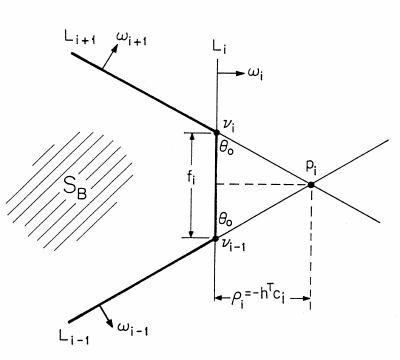
\includegraphics[width=10cm]{images/dicrete-radius-curvature.jpg}
    \caption{Иллюстрация к понятию дискретной кривизны.}
    \label{dicrete-radius-curvature}
\end{figure}

Далее в авторы развивают идею \textbf{дискретного радиуса кривизны} -- величины,
характеризующей гладкость поверхностей главных целей. Представим, что на
рисунке \ref{dicrete-radius-curvature} некоторая материальная точка движется
вдоль $i$-ой стороны многоугольника от экстремальной точки $\nu_{i - 1}$ до
другой экстремальной точки $\nu_{i}$. Тогда во время этого движения вектор
внешней нормали к поверхности меняет угол наклона на величину
$\theta_{0} = \theta_{i} - \theta_{i - 1}$. При этом точка преодолевает
расстояние, равное $f_{i}$. По аналогии с обычным радиусом кривизны,
определяемом как скорость заметания дуги радиусом-вектором поверхности по
отношению к углу наклона радиуса-вектора, авторы определяют дискретный радиус
кривизны как

\begin{equation}
r_{i} = \frac{f_{i}}{\theta_{0}}
\end{equation}

Из геометрических соображений можно показать, что расстояние от точки $p_{i}$
до прямой $L_{i}$ равно $\rho_{i} = -h^{T} c_{i}$, где $c_{i}$ -- $i$-й столбец
матрицы $C$, а из простого тригонометрического соотношения следует, что

\begin{equation}
f_{i} = \frac{2 \rho_{i}}{tg \theta_{0}}
\end{equation}

и, следовательно,

\begin{equation}
\rho_{i} = \frac{1}{2} r_{i} \theta_{0} tg \theta_{0}
\end{equation}

Отсюда следует, что вектор $\rho = - h^{T} C$ состоит из элементов,
пропорциональных дискретным радиусам кривизны $r_{i}$. При этом малые по
величине элементы этого вектора соответствуют "острым" углам, а большие --
"гладким". В дальнейшем авторы статьи используют это соображение в целях
конструирования объекта, гладкость которого известна заранее.

\subsubsection{Общие замечания об алгоритмах восстановления}

Всего Prince и Willsky приводят в статье 3 алгоритма для реконструкции выпуклого
тела по измерениям его опорной функции. При этом предполагается, что измерения
опорной функции получаются как

\begin{equation}
y_{i} = h_{i} + n_{i}, i = 1, \ldots, M
\end{equation}

где $h_{i}$ -- точные значения опорной функции, для которых требуется построить
оценку, а $n_{i}$ -- статистические погрешности, которые представляют собой

\begin{enumerate}
 \item Либо независимые одинаково распределенные гауссовы величины с нулевым
 средним и дисперсией $\sigma^{2}$
 \item Либо независимые случайные величины, равномерно распределенные на отрезке
 $[ - \gamma, \gamma]$.
\end{enumerate}

Вследствие наличия статистических погрешностей измерений нельзя утверждать, что
набор $y = (y_{1}, \ldots, y_{M})$ представляют из себя согласованный набор
опорных чисел. Поэтому первой задачей всех алгоритмов является построение
согласованного набора. Следующей задачей является построение такого
согласованного набора, который бы наилучшим образом соответствовал заранее
известной информации об измеряемом объекте.

\subsubsection{Алгоритм CLOSEST. Алгоритм ближайшего набора}
\label{sec:history/PrinceW90/algo-CLOSEST}

\textbf{Алгоритм ближайшего набора} представляет из себя следующее. В данном
случае предполагается, что статистические погрешности представляют собой
гауссовы величины. В случае, когда отсутствует какая-либо информация об
оцениваемом объекте, следует строить оценку максимального правдоподобия вектора
$h$ по вектору измерений $y$ при условии, что $h \in \mathfrak{C}$:

\begin{equation}
\widehat{h}_{C} = \widehat{h}_{ML} =
\operatornamewithlimits{argmax}_{h: h^{T} C \leq 0}
( - \frac{1}{2} (y - h)^{T} (y - h))
\end{equation}

Очевидно, что данная оценка предоставляет такой вектор $h$ из множества
$\mathfrak{C}$, который является наиболее близким к вектору измерений $y$ в
смысле евклидовой метрики. Если $y \in \mathfrak{C}$, то $\widehat{h}_{C} = y$,
в противном случае оценка $\widehat{h}_{C}$ может быть найдена методами
квадратичного программирования.

\subsubsection{Алгоритм MINI-MAX. Минимаксный алгоритм}


\textbf{Минимаксный алгоритм} предназначен для построения
оценки тела в случае, если заранее известно, что оно представляет из себя тело
с гладкой поверхностью. Для этого строится такая оценка, которая
\textit{максимизирует минимальный радиус кривизны} тела. В такой формулировке
решение всегда будет неограниченным, поскольку многоугольники, вписанные в
концентрические окружности неограниченно возрастающего радиуса, имеют
неограниченный дискретный радиус кривизны. Эту проблему можно решить, если
предположить, что статистические погрешности равномерно распределены на отрезке
$[ - \gamma, \gamma]$. В таком случае каждый реального вектора не может
отстоять от измеренной величины больше чем на $\gamma$. Из этого следует, что
реальный вектор и, следовательно, вектор оценки должен содержаться в гиперкубе

\begin{equation}
\mathfrak{B} = \{h \in \mathbb{R}^{M} |
y - [\gamma, \gamma, \ldots, \gamma]^{T} \leq h \leq
y + [\gamma, \gamma, \ldots, \gamma]^{T}\}
\end{equation}

Таким образом, поскольку величины $\rho_{i} = - h^{T} c_{i}$ пропорциональны
дискретным радиусам кривизны $r_{i}$, авторы статьи определяют минимаксную
оценку как

\begin{equation}
\widehat{h}_{MM} =
\operatornamewithlimits{argmax}_{h \in \mathfrak{C} \cap \mathfrak{B}}
\min_{i = 1, \ldots, M} ( - h^{T} c_{i})
\end{equation}

Решение этой задачи оптимизации может быть получено путем применения методов
линейного программирования. Чтобы показать это, введем новую скалярную величину,
удовлетворяющую следующим неравенствам:

\begin{equation}
\mu \leq - h^{T} c_{i}, i = 1, \ldots, M
\end{equation}

Затем рассмотрим расширенные векторы
$u = \left(
\begin{array}{c}
 h_{1} \\
 h_{2} \\
 \vdots \\
 h_{M} \\
 \mu \\
\end{array}
\right)$ и
$ b = \left(\begin{array}{c}
 0 \\
 0 \\
 \vdots \\
 0 \\
 1 \\
\end{array}
\right)$.

В таких обозначениях нетрудно заметить, что исходная задача может
быть переформулирована как максимизация величины $u^{T} b$ относительно
ограничений $\mu \leq - h^{T} c_{i}, i = 1, \ldots, M$. В такой формулировке и
функционал и неравенства ограничений линейны и, следовательно, задача
максимизации может быть решена методами линейного программирования.

Данный алгоритм наделен одним неудачным свойством: как это часто случается при
применении линейного программирования, решение задачи может быть не
единственным. Очевидно, что, например, прибавление произвольного вектора из ядра
$\mathfrak{N}$ матрицы $C$ не изменяет дискретные кривизны объекта и
следовательно, и функционал, максимизируемый в алгоритме. Следовательно, можно
утверждать, что решением задачи нахождения максиминной оценки является целое
семейство объектов, полученных из исходного методом плоскопараллельных сдвигов в
$\mathbb{R}^{2}$. Минимаксная оценка привязана к величинам, полученным из
измерений только внутри гиперкуба $\mathfrak{B}$, и поэтому при увеличении
$\gamma$ полученная минимаксная все меньше зависит от полученных из эксперимента
данных.

Поэтому минимаксный алгоритм всегда стремится построить многоугольник
наибольшего размера в рамках допустимого гиперкуба, причем этот многоугольник
всегда стремится к окружности. Такие результаты получаются даже если истинное
тело не обладает такими свойствами. Этот недостаток алгоритма послужил для
авторов статьи мотивацией к разработке еще одного алгоритма.

\subsubsection{Алгоритм CLOSE-MIN. Минимаксный алгоритм ближайшего набора}

\textbf{Минимаксный алгоритм ближайшего набора} изначально задуман таким
образом, чтобы скомбинировать алгоритм ближайшего набора и минимакный алгоритм.
Сделано это с целью, чтобы получаемая оценка с одной стороны максимально точно
приближала данные, полученные из измерений (как в первом алгоритме), а с другой
-- чтобы учесть заранее известные об объекте данные (как во втором алгоритме).
Идея метода предельно проста: максимизируемый функционал строится как выпуклая
комбинация функционалов двух алгоритмов. С точки зрения статистики алгоритм
представляет собой построение максимальной апостериорной оценки, при этом
слагаемое из алгоритма ближайшего набора играет роль логарифма плотности
измерений (TODO: разобраться в этих понятиях), а слагаемое из минимаксного
алгоритма играет роль логарифма первичной плотности.

Слагаемые берутся с коэффициентами соответственно $\alpha$ и $1 - \alpha$ для
того чтобы дать возможность для настройки алгоритма:

\begin{equation}
\widehat{h}_{CM} =
\operatornamewithlimits{argmax}_{h \in \mathfrak{C} \cap \mathfrak{B}}
(\alpha f_{C}(h) + (1 - \alpha) f_{M}(h))
\end{equation}

где $0 \leq \alpha \leq 1$ и $f_{C}(h)$ и $f_{M}(h)$ представляют из себя
функционалы из первых двух алгоритмов:

\begin{equation}
f_{C}(h) = - \frac{1}{2} (y - h)^{T} (y - h)
\end{equation}

\begin{equation}
f_{M}(h) = \min_{i = 1, \ldots, M} (- h^{T} c_{i})
\end{equation}

Решение данной задачи может быть найдено методами квадратичного
программирования путем расширения вектора $h$, как это было сделано в
минимаксном алгоритме. Заметим, что поскольку $\alpha \neq 0$, условие
принадлежности гиперкубу $\mathfrak{B}$ может быть опущено и решение задачи
является единственным.

\subsubsection{Модификация алгоритмов, учитывающая информацию о абсолютном
положении объекта}

Предположим, что заранее известно, что центр масс вершин некоторого объекта
расположен в точке $\overline{\nu}$. Тогда данная информация может быть также
заложена в процесс восстановления многоугольника -- восстановленный
многоугольник должен обладать таким же свойством. Данное условие может быть
достигнуто просто путем расширения набора ограничений еще одним линейным
равенством:

\begin{equation}
N^{T} h = \frac{M}{2} \overline{\nu}
\end{equation}

Вследствие линейности данного уравнения внесение его в число ограничений любого
из трех введенных выше алгоритмов не внесет качественных изменений в методы
работы этих алгоритмов (линейное и квадратичное программирование). Эффект от
добавления такого ограничения может быть довольно заметным.

\newpage
\subsection{Задача двумерного восстановления выпуклого тела по произвольно
распределенным измерениям опорной функции}

Дальнейшее развитие рассматриваемая проблема нашла в исследовании авторов Lele,
Kulkarni и Willsky, которое было описано в статье
\cite{journals/josaa/LeleKW92}. Более подробную информацию можно найти в
дипломной работе Lele \cite{thesis/Lele90}.

Данное исследование охватывает совершенно новую область применения --
распознание формы объектов по данным лазерного радара. В ней описано обобщение
первого алгоритма ближайшего набора Prince и Willsky для случая, когда
направления, по которым производится измерение опорной функции, распределены
произвольным образом. Также в ней вводится 2 новых алгоритма, которые позволяют
строить тело на основе априорной информации о количестве его сторон и
либо направлениях нормалей этих сторон, либо об относительных углах между этими
направлениями.

\subsubsection{Алгоритм NUA. Восстановление многоугольника со сторонами по
углам измерения}

Данный алгоритм является обобщением алгоритма ближайшего набора из статьи Prince
и Willsky, в котором тело строится по конечному набору величин
$y_{1}, y_{2}, \ldots, y_{M}$,  которые представляют собой измеренные с
погрешностями значениями опорной функции по направлениям вдоль известных углов
$\theta_{1} < \theta_{2} < \ldots < \theta_{M}$, которые называются
\textbf{углами измерения}. Отличие от упомянутого алгоритма состоит в том, что
критерий матрица в неравенстве из критерия согласованности записывается
несколько иным образом.

Тройка опорных чисел $h_{i - 1}, h_{i}, h_{i + 1}$ по углам $\theta_{i - 1},
\theta_{i}, \theta_{i + 1}$ является согласованной тогда и только тогда, когда
выполнено следующее неравенство:

\begin{equation}
h_{i - 1} sin(\theta_{i + 1} - \theta_{i}) -
h_{i} sin(\theta_{i + 1} - \theta_{i - 1}) +
h_{i + 1} sin(\theta_{i} - \theta_{i - 1}) \geq 0
\end{equation}

Опорная теорема теперь записывается следующим образом:

\begin{SmartTheorem}
 \label{thm:ext-support-theorem-2d}
 \textbf{Обобщенная двумерная опорная теорема}.
 Набор действительных чисел
 $h = (h_{1}, h_{2}, \ldots, h_{M}) \in \mathbb{R}^{M}$
 является набором опорных чисел по направлениям вдоль углов
 $\theta_{1} < \theta_{2} < \ldots < \theta_{M}$ тогда и только тогда, когда
 выполнено следующее матричное неравенство:

 \begin{equation}
 C h \geq 0
 \end{equation}

 где матрица $C$ представляет собой следующее:

 \begin{equation}
  \left(
  \begin{array}{ccccccc}

   \scriptstyle     -sin(\theta_{2} - \theta_{M}) &
   \scriptstyle     sin(\theta_{1} - \theta_{M}) &
   \scriptstyle     0 &
   \scriptstyle     \ldots &
   \scriptstyle     0 &
   \scriptstyle     0 &
   \scriptstyle     sin(\theta_{2} - \theta_{1}) \\

   \scriptstyle      sin(\theta_{3} - \theta_{2}) &
   \scriptstyle      -sin(\theta_{3} - \theta_{1}) &
   \scriptstyle      sin(\theta_{2} - \theta_{1}) &
   \scriptstyle      \ldots &
   \scriptstyle      0 &
   \scriptstyle      0 &
   \scriptstyle      0 \\

   \scriptstyle      0 &
   \scriptstyle      sin(\theta_{4} - \theta_{3}) &
   \scriptstyle      -sin(\theta_{4} - \theta_{2}) &
   \scriptstyle      \ldots &
   \scriptstyle      0 &
   \scriptstyle      0 &
   \scriptstyle      0 \\

   \scriptstyle      \vdots &
   \scriptstyle      \vdots &
   \scriptstyle      \vdots &
   \scriptstyle      \ddots &
   \scriptstyle      \vdots &
   \scriptstyle      \vdots &
   \scriptstyle      \vdots \\

   \scriptstyle      0 &
   \scriptstyle      0 &
   \scriptstyle      0 &
   \scriptstyle      \ldots &
   \scriptstyle      -sin(\theta_{M - 1} - \theta_{M - 3}) &
   \scriptstyle      sin(\theta_{M - 2} - \theta_{M - 3}) &
   \scriptstyle      0 \\

   \scriptstyle      0 &
   \scriptstyle      0 &
   \scriptstyle      0 &
   \scriptstyle      \ldots &
   \scriptstyle      sin(\theta_{M} - \theta_{M - 1}) &
   \scriptstyle      -sin(\theta_{M} - \theta_{M - 2}) &
   \scriptstyle      sin(\theta_{M - 1} - \theta_{M - 2}) \\

   \scriptstyle      sin(\theta_{M} - \theta_{M - 1}) &
   \scriptstyle      0 &
   \scriptstyle      0 &
   \scriptstyle      \ldots &
   \scriptstyle      0 &
   \scriptstyle      sin(\theta_{1} - \theta_{M}) &
   \scriptstyle      -sin(\theta_{1} - \theta_{M - 1}) \\
  \end{array}
  \right)
 \end{equation}
\end{SmartTheorem}

Данный алгоритм авторы называют NUA (от nonuniform angles).

\subsubsection{Алгоритм BNGON. Наилучший N-угольник по M измерениям с заданными
углами восстановления}

Данный алгоритм был разработан для случая, когда известна следующая априорная
информация об объекте: точное количество сторон многоугольника и углы наклона
нормалей к этим сторонам (эти углы далее будут называться \textbf{углами
восстановления}). Такая информация позволяет получать более качественную оценку
многоугольника.

Обозначим углы измерений через $\{\theta_{1}, \theta_{2}, \ldots,
\theta_{M}\}$, величины приближенно измеренных опорных чисел через $\{y_{1},
y_{2}, \ldots, y_{M}\}$, а известные углы восстановления через $\{\phi_{1},
\phi_{2}, \ldots, \phi_{N}\}$. По этим данным требуется построить N-угольник,
определяемый  согласованным набором опорных чисел $\{h_{\phi}(\phi_{1}),
h_{\phi}(\phi_{2}), \ldots, h_{\phi}(\phi_{N})\}$ по заданным углам
восстановления, который доставляет минимум для следующего функционала:

\begin{equation}
J[h_{\phi}(\phi_{1}), h_{\phi}(\phi_{2}), \ldots, h_{\phi}(\phi_{N})] =
\sum \limits_{i = 1}^{M}[h_{\phi}(\theta_{i}) - y_{i}]^{2}
\end{equation}

Как известно, опорная функция многоугольника представляет собой
кусочно-синусоидальную функцию. Поэтому значения $h_{\phi}(\theta_{i})$ всегда
можно вычислить следующим образом:

\begin{enumerate}
 \item Найти соседние углы восстановления $\phi_{L_{i}}$ и $\phi_{R_{i}}$
такие, что $\phi_{L_{i}} < \theta_{i} < \phi_{R_{i}}$ и на отрезке
$[\phi_{L_{i}}, \phi_{R_{i}}]$ нет других углов восстановления.
 \item Вычислить $h_{\phi}(\theta_{i})$ по следующей формуле:
\end{enumerate}

\begin{equation}
h_{\phi}(\theta_{i}) =
\frac{sin(\phi_{R_{i}} - \theta_{i})}{sin(\phi_{R_{i}} - \phi_{L_{i}})}
h_{L_{i}} +
\frac{sin(\theta_{i} - \phi_{L_{i}})}{sin(\phi_{R_{i}} - \phi_{L_{i})}}
h_{R_{i}}
\end{equation}

Используя это соотношение, задачу минимизации можно переформулировать следующим
образом:

\begin{equation}
\widehat{h}_{\phi} = \left(
\begin{array}{c}
 \widehat{h}_{\phi}(\phi_{1}) \\
 \widehat{h}_{\phi}(\phi_{2}) \\
 \vdots \\
 \widehat{h}_{\phi}(\phi_{N}) \\
\end{array}
\right) = \operatornamewithlimits{argmin}_{C h_{\phi} \geq 0} (A h_{\phi} -
y)^{T} (A h_{\phi} - y)
\end{equation}

где $A$ есть $M \times N$ матрица, строками которой являются коэффициенты
линейных комбинаций элементов вектора $h_{\phi} = [h_{\phi}(\phi_{1})c,
h_{\phi}(\phi_{2}), \ldots, {\phi}(\phi_{N})]^{T}$, через которые
выражаются соответствующие опорные числа $h_{\phi}(\theta_{1}),
h_{\phi}(\theta_{2}), \ldots, h_{\phi}(\theta_{M})$ по углам измерений.

Поскольку рассматриваемый функционал является квадратичным, а ограничения на
условия минимизации являются линейными, искомый минимум может быть найден с
помощью стандартных методов квадратичного программирования.

В статье авторы называют этот алгоритм BNGON (best N-gon).

\subsubsection{Алгоритм BNGONROT. Наилучший N-угольник по M измерениям с
заданными относительными углами}

Данный алгоритм предназначен для случая, когда о теле доступна несколько
меньшая информация, а именно известны относительные углы между нормалями, но
абсолютные значения этих углов неизвестны.

Пусть как и раньше $\{\theta_{1}, \theta_{2}, \ldots,
\theta_{M}\}$ суть углы измерений, а величины приближенно измеренных опорных
чисел суть $\{y_{1}, y_{2}, \ldots, y_{M}\}$. Отличие от предыдущего алгоритма
состоит в том, что углами восстановления являются $\{\phi_{1} + \alpha,
\phi_{2} + \alpha, \ldots, \phi_{N} + \alpha\}$, где $\{\phi_{1}, \phi_{2},
\ldots, \phi_{N}\}$ известны, а $\alpha \in [0, 2 \pi]$ служит неизвестным
смещением углов восстановления.

Минимизируемым функционалом в данном случае является

\begin{equation}
J[\alpha, h_{\phi}(\phi_{1} + \alpha), h_{\phi}(\phi_{2} + \alpha), \ldots,
h_{\phi}(\phi_{N} + \alpha)] =
\sum \limits_{i = 1}^{M}[h_{\phi}(\theta_{i}) - y_{i}]^{2}
\end{equation}

причем величины $h_{\phi}(\theta_{i})$ вычисляются по похожей формуле

\begin{equation}
h_{\phi}(\theta_{i}) =
\frac{sin(\phi_{R_{i}} + \alpha - \theta_{i})}{sin(\phi_{R_{i}} - \phi_{L_{i}})}
h_{L_{i}} +
\frac{sin(\theta_{i} - \phi_{L_{i}} - \alpha)}{sin(\phi_{R_{i}} - \phi_{L_{i})}}
h_{R_{i}}
\end{equation}

Однако данный функционал не является квадратичным вследствие того, что
неизвестная $\alpha$ входит в выражение через аргументы тригонометрических
функций. Тем не менее, авторы приводят основанный на квадратичном
программировании алгоритм, который позволяет решить эту задачу.

Обозначим через $J_{h_{\phi}}(\alpha)$ минимум функционала по значениям опорных
чисел при фиксированном значении смещения $\alpha$.

\begin{equation}
J_{h_{\phi}}(\alpha) = \min_{{h_{\phi}(\phi_{i} + \alpha)}} J[\alpha,
h_{\phi}(\phi_{1} + \alpha), h_{\phi}(\phi_{2} + \alpha), \ldots,
h_{\phi}(\phi_{N} + \alpha)]
\end{equation}

Самым простым решением данной задачи является решение методом грубой
силы: перебор некоторого большого набора величин смещений $\alpha$, взятых с
определенным шагом. Такой подход является, без сомнения, довольно трудоемким.
Поэтому авторы разработали более эффективный градиентный алгоритм. Сущность
задачи внесла два важных отличия в этот алгоритм по сравнению с обычным
алгоритмом градиентного спуска. Во-первых, заметим что

\begin{equation}
J_{h_{\phi}}(\alpha) = J[\alpha,
h_{\phi}^{*}(\phi_{1} + \alpha), h_{\phi}^{*}(\phi_{2} + \alpha), \ldots,
h_{\phi}^{*}(\phi_{N} + \alpha)]
\end{equation}

где величины $h_{\phi}^{*}(\phi_{i} + \alpha)$ доставляют минимум для
функционала $J_{h_{\phi}}(\alpha)$. Поэтому

\begin{equation}
\frac{d J_{h_{\phi}}(\alpha)}{d \alpha} = \frac{\partial J}{\partial \alpha} +
\sum \limits_{i = 1}^{N} \frac{\partial J}{\partial h_{\phi}(\phi_{i} + \alpha)}
\frac{\partial h_{\phi}^{*}(\phi_{i} + \alpha) }{\partial \alpha}
\end{equation}

Здесь вычисление величины
$\frac{\partial h_{\phi}^{*}(\phi_{i} + \alpha)}{\partial \alpha}$ представляет
большую трудность, поскольку вычисление каждого значения
$h_{\phi}^{*}(\phi_{i} + \alpha)$ требует решения задачи квадратичного
программирования. Поэтому авторы приняли решение использовать в градиентном
методе не полную, а лишь частную производную:

\begin{equation}
\frac{\partial J}{\partial \alpha} [\alpha,
h_{\phi}^{*}(\phi_{1} + \alpha), h_{\phi}^{*}(\phi_{2} + \alpha), \ldots,
h_{\phi}^{*}(\phi_{N} + \alpha)] =
2 \sum \limits_{i = 1}^{M}  \frac{\partial h_{\phi}(\theta_{i}) }{\partial
\alpha} [h_{\phi}^{*}(\theta_{i}) - y(\theta_{i})]
\end{equation}

где используя известное выражение для опорных чисел в углах измерения через
опорные числа в углах восстановления можно получить:

\begin{equation}
\frac{\partial h_{\phi}(\theta_{i})}{\partial \alpha} =
\frac{cos(\phi_{R_{i}} + \alpha - \theta_{i})}{sin(\phi_{R_{i}} - \phi_{L_{i}})}
h_{L_{i}} +
\frac{cos(\theta_{i} - \phi_{L_{i}} - \alpha)}{sin(\phi_{R_{i}} - \phi_{L_{i})}}
h_{R_{i}}
\end{equation}

Вторым важным отличием представленного алгоритма является то, что функция
$J_{h_{\phi}}(\alpha)$ является, вообще говоря, сильно невыпуклой функцией от
$\alpha$ (авторы отсылают на \cite{thesis/Lele90}, где этот вопрос рассмотрен
более детально). Данный факт приводит к тому, что для решения задачи нужно
найти все возможные локальные минимумы функционала. Авторы предлагают делать это
следующим образом.

\begin{enumerate}
 \item Положить $\alpha = 0$.
 \item Вычислить $\frac{\partial J}{\partial \alpha}$.
 \item Если $\frac{\partial J}{\partial \alpha} > 0$, сделать шаг градиентного
подъема, в противном случае -- шаг градиентного спуска.
 \item Если изменение величины функционала не превышает заданный порог
$\epsilon$, то сообщить о найденном локальном минимуме и перейти к шагу 7.
 \item Если знак функционала не поменялся, вернуться к шагу 2
 \item Если знак функционала поменялся, то методом деления пополам найти точку
изменения знака и сообщить, что в ней есть локальный минимум.
 \item Если $\alpha < 2 \pi$, увеличить $\alpha := \alpha + \delta \alpha$ и
вернуться к шагу 2 для того, чтобы найти еще один локальный минимум. В противном
случае завершить алгоритм.
\end{enumerate}

Затем нужно найти оптимальный минимум среди сообщенных данным алгоритмом.

В статье авторы называют этот алгоритм BNGONROT (best N-gon with rotations).

\newpage
\subsection{Задача трехмерного восстановления выпуклого тела по произвольно
распределенным измерениям опорной функции}

В данном разделе приводятся результаты статей \cite{journals/jmiv/KarlKVW96} и
\cite{conf/spie/GregorR2001}, целью которых было обобщить имеющиеся методы на
трехмерный случай. В первой статье приведен математический аппарат алгоритма,
а во второй -- описана его реализация и приведены результаты практических
вычислений. Стоит заметить, что время работы алгоритма оказалось довольно
большим, и возможно это послужило причиной тому, что он не получил широкое
распространение. В текущей работе приводятся идеи, каким образом можно сильно
увеличить производительность алгоритма: как в общем, так и в частном случае
для практической задачи восстановления по теневым контурам.

Основным предметом исследования статьи \cite{journals/jmiv/KarlKVW96} является
поиск набора условий, являющийся критерием согласованности набора измерений
опорной функции произвольного выпуклого тела в $\mathbb{R}^{N}$. Новизна статьи
состоит в том, что задача рассматривается для случая произвольной размерности.
При этом авторы строят набор условий, исходя из их практической применимости в
реальных алгоритмах восстановления.

\subsubsection{Критерий опорной функции в $\mathbb{R}^{n}$}

Довольно естественным вопросом, который возникает пр рассмотрении опорных
функций является следующий: какие функции могут быть опорными для некоторого
тела? Ответ на этот вопрос дает следующая классическая теорема:

\begin{SmartTheorem}
 \label{thm:support-function-criterio-R2}
 \textbf{Критерий опорной функции}.
 Функция $H(v): \mathbb{R}^{2} \to \mathbb{R}$ является опорной функцией
 некоторого выпуклого тела тогда и только когда она определена на всем
 $\mathbb{R}^{n}$ и удовлетворяет следующим свойствам:
 \begin{enumerate}
  \item $H(0) = 0$.
  \item $H(\alpha v) = \alpha H(v)$ для всех $\alpha > 0$.
  \item $H(v + w) \leq H(v) + H(w)$ для всех $v, w \in \mathbb{R}^{n}$
 \end{enumerate}
\end{SmartTheorem}

Впервые доказательство данной теоремы было представлено Минковским для случая
трехмерной размерности, а позже в работе \cite{journals/mz/Rademacher22}
Радемахером было произведено обобщение на случай произвольной размерности.
Неудобство этой теоремы с точки зрения приложений состоит в том, что условие,
которое ей формулируется, является \textit{глобальным}, в том смысле, что оно
должно быть проверяемо для каждой пары векторов $v$ и $w$ в $\mathbb{R}^{n}$.

Потому Радемахер показал, что 3-е условие теоремы может быть заменено другим.
А именно, было показано, что при условиях 1 и 2 теоремы
\ref{thm:support-function-criterio-R2} условие 3 эквивалентно следующему:

\begin{SmartTheorem}
 \label{thm:support-function-criterio-R2-det}
 \textbf{Детерминантный критерий опорной функции}.
 Функция $H(v): \mathbb{R}^{2} \to \mathbb{R}$ является опорной функцией
 некоторого выпуклого тела тогда и только когда выполнены условия 1 и 2 из
 теоремы \ref{thm:support-function-criterio-R2} а также следующее условие:

\begin{equation}
 \left|\begin{array}{cc}
  h(u_{1}) & u_{1}^{T} \\
  h(u_{2}) & u_{2}^{T} \\
  h(u_{3}) & u_{3}^{T} \\
 \end{array}\right|
  \left|\begin{array}{cc}
  1 & u_{1}^{T} \\
  1 & u_{2}^{T} \\
  1 & u_{3}^{T} \\
 \end{array}\right|
 \geq 0
\end{equation}
для всевозможных троек единичных векторов $u_{1}, u_{2}, u_{3}$.
\end{SmartTheorem}

Теперь в отличие данной теоремы от критерия опорной функции (см. теорему
\ref{thm:support-function-criterion}) состоит в том, что она не требует
дифференцируемости, но формулирует условие прямо в терминах
\textit{экспериментально измеряемых величин} $h(u)$.

Предположим, что все числа $u_{1}$, $u_{2}$, $u_{3}$ различны и что $u_{3}$
лежит в либо в положительной, либо в отрицательной части конуса для точек
$\{u_{1}, u_{2}\}$ (этого условия можно достичь просто путем переименования
переменных).

Также авторы статьи показывают, что последнее условие теоремы
\ref{thm:support-function-criterio-R2-det} эквивалентно следующему:

\begin{equation}
 \beta \left( u_{3}^{T}
 \left[
 \begin{array}{c}
 u_{1}^{T} \\
 u_{2}^{T} \\
 \end{array}
 \right]^{-1}
 \left[
 \begin{array}{c}
 h(u_{1}) \\
 h(u_{2}) \\
 \end{array}
 \right] - h(u_{3}) \right) \geq 0
\end{equation}

где скалярная функция $\beta = \beta(u_{1}, u_{2}, u_{3})$ зависит только от
набора чисел $u_{i}$. При этом если $u_{3}$ лежит в положительном конусе для
$\{u_{1}, u_{2}\}$, то $\beta(u_{1}, u_{2}, u_{3}) \geq 0$, а если в
отрицательном -- то $\beta(u_{1}, u_{2}, u_{3}) < 0$.

Однако данные условия все еще являются глобальными, поскольку требуют проверки
по всем возможным тройкам единичных векторов $(u_{1}, u_{2}, u_{3})$.

Результат Радемахера был обобщен на случай произвольной размерности:

\begin{SmartTheorem}
 \label{thm:support-function-criterio-ext}
 \textbf{Обобщенный критерий опорной функции}.
 Функция $H(v): \mathbb{R}^{n} \to \mathbb{R}$ является опорной функцией
 некоторого выпуклого тела в $\mathbb{R}^{n}$ тогда и только когда она
 определена на всем $\mathbb{R}^{n}$ и удовлетворяет следующим свойствам:
 \begin{enumerate}
  \item $H(0) = 0$.
  \item $H(\alpha v) = \alpha H(v)$ для всех $\alpha > 0$.
  \item Следующее детерминантное неравенство выполняется для каждого набора из
  $n + 1$ единичных векторов $u_{i}$, в котором один из векторов лежит в полном
  положительном конусе основных:
\begin{equation}
\label{thm:support-function-criterio-ext:condition}
 \left|\begin{array}{cc}
  h(u_{1}) & u_{1}^{T} \\
  h(u_{2}) & u_{2}^{T} \\
  \vdots & \vdots \\
  h(u_{n + 1}) & u_{n + 1}^{T} \\
 \end{array}\right|
  \left|\begin{array}{cc}
  1 & u_{1}^{T} \\
  1 & u_{2}^{T} \\
  \vdots & \vdots \\
  1 & u_{n + 1}^{T} \\
 \end{array}\right|
 \geq 0
\end{equation}

 \end{enumerate}
\end{SmartTheorem}

Точно так же, как и в плоском случае, можно показать, что последнее неравенство
эквивалентно следующему:

\begin{equation}
\label{thm:support-function-criterio-ext:condition2}
 u_{n + 1}^{T}
 \left[
 \begin{array}{c}
 u_{1}^{T} \\
 u_{2}^{T} \\
 \vdots \\
 u_{n}^{T} \\
 \end{array}
 \right]^{-1}
 \left[
 \begin{array}{c}
 h(u_{1}) \\
 h(u_{2}) \\
 \vdots \\
 h(u_{n}) \\
 \end{array}
 \right] - h(u_{n + 1}) \geq 0
\end{equation}

\subsubsection{Критерий набора опорных чисел в $\mathbb{R}^{n}$}

Как упоминалось ранее, измерения опорной функции, которые получаются из
экспериментальных данных, содержат погрешности, которые приводят к тому, что
набор перестает быть согласованным. Чтобы восстановить согласованность набора,
нужно ввести ряд условий, который будет задавать множество всех наборов опорных
чисел.

\begin{SmartTheorem}
 \label{thm:discrete-consistency}
 \textbf{Критерий набора опорных чисел в $\mathbb{R}^{n}$}.
 Набор действительных чисел $h = (h_{1}, h_{2}, \ldots, h_{N})$ по
 направлениям $u_{1}, u_{2}, \ldots, u_{N}$ является набором  опорных чисел
 некоторого выпуклого тела в $\mathbb{R}^{n}$ тогда и только тогда, когда
 каждый поднабор $h_{(i_{1}, i_{2}, \ldots i_{n + 1})} = \{h_{i_{1}}, h_{i_{2}},
 \ldots, h_{i_{n + 1}}\}$ из $n + 1$ чисел удовлетворяет следующему условию:

 Для каждого числа $h_{i_{j}}$ из $(n + 1)$-поднабора гиперплоскость,
 соответствующая числу, имеет непустое пересечение с пересечением всех $n + 1$
 соответствующих полупространств:

 \begin{equation}
 \label{thm:discrete-consistency:condition}
  \pi(h_{i_{j}}, u_{i_{j}}) \cap \bigcap \limits_{k = 1}^{n + 1} R(h_{i_{k}},
  u_{i_{k}}) \neq \varnothing \;\;\; \forall j = 1, 2, \ldots, n + 1
 \end{equation}

 где через
 $\pi(h, u) = \{x \in \mathbb{R}^{n} \; | \; (x, u) = h\}$
 обозначается  гиперплоскость, а через
 $R(h, u) = \{x \in \mathbb{R}^{n} \; | \; (x, u) \leq h\}$
 -- полупространство, соответствующие опорному числу $h$ по направлению $u$.
\end{SmartTheorem}

Фактически последнее условие является обобщением геометрической интерпретации,
изображенной на рис. \ref{dicrete-radius-curvature}. Недостаток данной теоремы
с точки зрения приложений состоит в том, что условие должно быть проверено для
всех возможных $(n + 1)$-поднаборов, т. е. оно не является \textit{локальным}.
Вследствие этого авторы посвятили оставшуюся часть статьи сокращению числа
условий, которые должны быть проверены.

\subsubsection{Локальный критерий набора опорных чисел в $\mathbb{R}^{n}$}

Главным результатом статьи является сокращение числа условий до того, что
критерий становится локальным. Во-первых, проводится классификация $(n +
1)$-поднаборов:

\begin{SmartDefinition}
 \label{def:tuples-classifiction}
 Пусть имеется набор $(u_{1}, u_{2}, \ldots, u_{n + 1})$ из $n + 1$ векторов в
 $\mathbb{R}^{n}$. Тогда он называется
 \begin{enumerate}
  \item \textbf{конусно-положительным}, если один из векторов $u_{i}$
  положительной конусной оболочке остальных.
  \item \textbf{конусно-отрицательным}, если один из векторов $u_{i}$
  отрицательной конусной оболочке остальных.
  \item \textbf{конусно-нейтральным} -- в противном случае.
 \end{enumerate}
\end{SmartDefinition}

Последний класс наборов -- конусно-нейтральный -- не представляет интереса для
исследования, поскольку в нем условие \ref{thm:discrete-consistency:condition}
из теоремы \ref{thm:discrete-consistency} выполняется автоматически. Более
того, при условии что
$\bigcap \limits_{i = 1}^{N} R(h_{i}, u_{i}) \neq \varnothing$,
т. е. пересечение всех соответствующих опорным числам полупространств непусто,
условие \ref{thm:discrete-consistency:condition} выполняется автоматически и
для конусно-отрицательных наборов.

Далее, если конусно-положительный набор является невырожденным, т. е.
соответствующая конусная оболочка является \textit{полной}, то условие
\ref{thm:discrete-consistency:condition} из теоремы
\ref{thm:discrete-consistency} эквивалентно детерминантному условию
\ref{thm:support-function-criterio-ext:condition} из теоремы
\ref{thm:support-function-criterio-ext}, или эквивалентному ему матричному
условию \ref{thm:support-function-criterio-ext:condition2}.

Данные соображения используются для введения следующего критерия:

\begin{SmartTheorem}
 \label{thm:positive-cone-consistency}
 \textbf{Конусно-положительный критерий набора опорных чисел в $\mathbb{R}^{n}$}
 Пусть имеется набор действительных чисел $h = (h_{1}, h_{2}, \ldots, h_{N})$ по
 направлениям $u_{1}, u_{2}, \ldots, u_{N}$. Пусть выполнены следующие
 условия:
 \begin{enumerate}
  \item Пересечение всех соответствующих полупространств непусто:
  \begin{equation}
   \bigcap \limits_{i = 1}^{N} R(h_{i}, u_{i}) \neq \varnothing
  \end{equation}
  \item Для каждого конусно-положительного $(n + 1)$-поднабора конусная оболочка
  является полной.
 \end{enumerate}

 Тогда данный набор является набором опорных чисел некоторого выпуклого тела в
 $\mathbb{R}^{n}$ тогда и только тогда, когда условие
 \ref{thm:support-function-criterio-ext:condition} из теоремы
 \ref{thm:support-function-criterio-ext} выполняется для каждого
 конусно-положительного $(n + 1)$-поднабора чисел.
\end{SmartTheorem}

Далее авторы статьи с помощью идеи, которую они называют \textbf{слиянием
согласованности}, проводят сведение глобального критерия согласованности к
локальному:

\begin{SmartLemma}
 \label{lem:consistency-merging}
 \textbf{Слияние согласованности}.
 Пусть имеется множество из $(n + 2)$ опорных чисел $h_{i}$ по направлениям
 $u_{i}$ в $\mathbb{R}^{n}$ и пусть выполнены следующие условия:

 \begin{enumerate}
  \item $u_{n + 1} \in cone^{+}\{u_{1}, \ldots, u_{n - 1}, u_{n + 2}\}$
  \item $u_{n + 2} \in cone^{+}\{u_{2}, \ldots, u_{n}, u_{n + 1}\}$
  \item $\{u_{n + 1}, u_{n + 2}\} \in cone^{+}\{u_{1}, \ldots, u_{n - 1},
u_{n}\}$
  \item Все три этих конуса являются полными.
 \end{enumerate}

 Тогда если наборы опорных чисел
 $\{h_{1}, \ldots, h_{n - 1}, h_{n + 1}, h_{n + 2}\}$ и
 $\{h_{2}, \ldots, h_{n}, h_{n + 1}, h_{n + 2}\}$ согласованы, то и наборы
 $\{h_{1}, \ldots, h_{n}, h_{n + 1}\}$ и
 $\{h_{1}, \ldots, h_{n}, h_{n + 2}\}$ также являются согласованными.
\end{SmartLemma}

Для того, чтобы конкретизировать понятие \textit{локальности}, авторы статьи
вводят следующее определение:

\begin{SmartDefinition}
 \label{def:local-family}
 \textbf{Локальное семейство}.
 Пусть имеется набор $\mathit{S}$ из $m$ различных единичных векторов в
 $\mathbb{R}^{n}$. Пусть $u_{k}$ - один из этих векторов. Тогда
 \textbf{локальным семейством}, соответствующим вектору $u_{k}$, называется
 множество всех различных $(n + 1)$-поднаборов $u_{i_{1}, \ldots,
 i_{n}} = \{u_{k}, u_{i_{1}}, u_{i_{2}}, \ldots, u_{i_{n}}\}$ векторов из
 $\mathit{S}$ таких,
 что:
 \begin{enumerate}
  \item $u_{k}$ является элементом этого $(n + 1)$-поднабора (это видно и по
  определению этого поднабора как $u_{i_{1}, \ldots,
 i_{n}} = \{u_{k}, u_{i_{1}}, u_{i_{2}}, \ldots, u_{i_{n}}\}$).
  \item Полная положительная конусная оболочка векторов $\{u_{i_{1}},
  u_{i_{2}}, \ldots, u_{i_{n}}\}$ содержит векторы $u_{k}, u_{i_{1}}, u_{i_{2}},
  \ldots, u_{i_{n}}$ и не содержит никаких других векторов из $\mathit{S}$.
 \end{enumerate}
\end{SmartDefinition}

Основным результатом статьи является следующая теорема, которая представляет
собой локальный критерий согласованности набора опорных чисел:

\begin{SmartTheorem}
 \label{thm:local-global-consistency-equivalence}
 \textbf{Локальный критерий набора опорных чисел в $\mathbb{R}^{n}$}.
 Пусть имеется набор действительных чисел $h = (h_{1}, h_{2}, \ldots, h_{N})$ по
 направлениям $u_{1}, u_{2}, \ldots, u_{N}$. Пусть выполнены следующие
 условия:
 \begin{enumerate}
  \item Пересечение всех соответствующих полупространств непусто:
  \begin{equation}
   \bigcap \limits_{i = 1}^{N} R(h_{i}, u_{i}) \neq \varnothing
  \end{equation}
  \item Для каждого конусно-положительного $(n + 1)$-поднабора конусная оболочка
  является полной.
 \end{enumerate}

 Тогда данный набор является набором опорных чисел некоторого выпуклого тела в
 $\mathbb{R}^{n}$ тогда и только тогда, когда условие
 \ref{thm:support-function-criterio-ext:condition} из теоремы
 \ref{thm:support-function-criterio-ext} выполняется для каждого направляющего
 вектора $u_{k}$ опорные числа $\{h_{k}, h_{i_{1}}, \ldots, h_{i_{n}}\}$,
 соответствующие направлениям $\{u_{k}, u_{i_{1}}, \ldots, h_{u_{n}}\}$ из
 локального семейства $u_{k}$.
\end{SmartTheorem}

Таким образом, результаты Prince и Willsky из
статьи \cite{journals/pami/PrinceW90}, который рассмотрен в разделе
\ref{sec:history/PrinceW90}, можно расширить на случай задач произвольной
размерности. Пусть $t = |\bigcup \limits_{i = 1}^{N} LF_{i}|$ - число элементов
локальных семейств всех направлений (через $LF_{i}$ обозначено $i$-е локальное
семейство). Тогда можно сформулировать все те задачи минимизации, которые
рассматривали Prince и Willsky, с тем лишь отличием, что вместо условия
$Ch \leq 0$ должно быть использовано условие

\begin{equation}
 Q h \geq 0
\end{equation}

где $Q$ -- $t \times m$ матрица, составленная из коэффициентов линейных
комбинаций условий согласованности для каждого набора из каждого локального
семейства. При этом каждая строка этой матрицы содержит не более $n + 1$
ненулевых коэффициентов.

\subsubsection{Алгоритм Gregor -- Rannou, основанный на критерии
согласованности}

Алгоритмы оптимизации, предложенные Karl, Kulkarni, Verghese, Willsky в статье
\cite{journals/jmiv/KarlKVW96}, как кажется, до сих пор еще не нашли применения
в крупных производственных системах. Единственной известной на
сегодняшний день попыткой является применение данного метода для построения
оценки трехмерной опорно функции к задаче магнитно-резонансной визуализации,
которое было произведено Gregor и Rannou. Результаты их работы были
опубликованы в статье \cite{journals/ijist/GregorR2002} и в материалах
конференции \cite{conf/spie/GregorR2001}. Здесь мы не будем описывать
проблемы, специфичные для магнитно-резонансной визуализации, поскольку в
конечном счете Gregor и Rannou свели свою задачу к аналогичным задачам,
обсуждавшимся выше.

\subsubsection{Тесты на согласованность}

Авторы в данной работы сделали некоторые упрощения в выражениях типа
\ref{thm:support-function-criterio-ext:condition}, используемых в качестве
условий минимизации функционала. Повторим ряд введенных определений (здесь для
ясности и связи с контекстом текущей работы мы несколько видоизменили ряд
определений и обозначений).

\begin{SmartDefinition}
 \label{def:cone}
 \textbf{Конусом} называется произвольная тройка векторов
 $\{u_{1}, u_{2}, u_{3}\} \subset \mathbb{R}^{3}$.
\end{SmartDefinition}

\begin{SmartDefinition}
 \label{def:full-cone}
 Конус называется \textbf{полным}, если его векторы линейно независимы.
\end{SmartDefinition}

\begin{SmartDefinition}
 \label{def:full-positive-cone}
 \textbf{Положительным конусом} векторов $u_{1}, u_{2}, u_{3}$ называется
 коническая оболочка этих векторов:

 \begin{equation}
  cone^{+}(u_{1}, u_{2}, u_{3}) =
  \{x = \alpha_{1} u_{1} + \alpha_{2} u_{2} + \alpha_{3} u_{3}
  \; | \; \alpha_{1} \geq 0, \alpha_{2} \geq 0, \alpha_{3} \geq 0\}
 \end{equation}
\end{SmartDefinition}

Вектор $u \in \mathbb{R}^{3}$ находится в положительном конусе, образованном
векторами $u_{1}, u_{2}, u_{3}$, когда он представим в следующем виде:

\begin{equation}
 u = \sum \limits_{i = 1}^{3} w_{i} u_{i}
\end{equation}

где $w = F^{-1} u \geq 0$ и $F = [u_{1}, u_{2}, u_{3}]$ - матрица, составленная
из векторов $u_{1}, u_{2}, u_{3}$.

\begin{SmartTheorem}
 \label{thm:criterion-gregor-rannou}
 \textbf{Критерий набора опорных чисел в форме Gregor, Rannou}.
 Набор $h = (h_{1}, h_{2}, \ldots, h_{N})$ действительных чисел является набором
 опорных чисел по направлениям $u_{1}, u_{2}, \ldots, u_{N}$ тогда и только
 тогда, когда для каждой четверки направлений
 $\{u_{i}, u_{i_{1}}, u_{i_{2}}, u_{i_{3}}\}$,
 для которой верно, что $u_{i} \in cone^{+}(u_{i_{1}}, u_{i_{2}}, u_{i_{3}})$,
 причем $u_{i} = \sum \limits_{j = 1}^{3} w_{i} u_{i_{j}}$, выполняется
 следующее соотношение:

 \begin{equation}
  \label{thm:criterion-gregor-rannou:condition}
  h_{i} - \sum \limits_{j = 1}^{3} w_{i} h_{i_{j}} \leq 0
 \end{equation}
\end{SmartTheorem}

Условия вида \ref{thm:criterion-gregor-rannou:condition} и будут образовывать
условия минимизации. Проверить их все невозможно, поэтому авторы обратились к
методам, предложенным в статье \cite{journals/jmiv/KarlKVW96} для снижения числа
этих условий. А именно, в условия минимизации предлагается включать только те
тесты, которые проверяют согласованность по локальным семействам (см.
определение \ref{def:local-family}).

\subsubsection{Формулировка задачи минимизации}

Пусть $t$ - общее число тестов на согласованность, которые необходимо проверить
для доказательства согласованности набора опорных чисел по заданным
направлениям $u_{1}, u_{2}, \ldots, u_{N}$. Тогда обозначим матрицу $Q$ как
$t \times N$ матрицу, составленную из коэффициентов отношений
\ref{thm:criterion-gregor-rannou:condition}. Данная матрица является сильно
разреженной, поскольку в каждой строке она содержит только 4 ненулевых элемента.
Пусть $h^{0}$ - начальное приближение набора опорных чисел (т. е. полученное из
эксперимента). Тогда ближайший к нему согласованный набор опорных чисел (в
смысле евклидовой нормы) может быть найден как решение следующей задачи
минимизации:

\begin{equation}
 \label{eq:gregor-rannou-algorithm}
 h^{*} = \operatornamewithlimits{argmin}_{\{h \; | \; Q h \leq 0\}}
 \frac{1}{2} ||h - h^{0}||^{2}
\end{equation}

В первую очередь авторы вычисляют матрицу $Q$ и дают представление об алгоритме,
решающем поставленную задачу минимизации.

\subsubsection{Построение матрицы $Q$}

Прежде всего следует заметить, что авторы используют для тестирования своего
алгоритма набор направлений, который заранее фиксирован. Этот набор направлений
обладает тем свойством, что векторы распределены равномерно с некоторым шагом по
поверхности единичной сферы $S_{2} \subset \mathbb{R}^{3}$. Набор наделен такими
свойствами инвариантности относительно поворота на угол $\frac{\pi}{2}$ и
отражений относительно некоторой плоскости. Это дает возможность снизит
количество необходимых вычислений в 8 раз. Обозначая через матрицу

\begin{equation}
 [u_{i_{1}}, u_{i_{2}}, u_{i_{3}}] = F^{-1} = [f_{ij}]
\end{equation}

обратную матрицу к матрице из координат векторов $u_{i{1}}, u_{i{2}}, u_{i{3}}$,
авторы формулируют соотношение, которое нужно проверить для того, чтобы
утверждать, что данная тройка векторов содержит вектор
$u_{i} = [sin \theta cos \phi, sin \theta sin \phi, cos \theta]^{T}$
в своем положительном конусе:

\begin{equation}
 \left[
 \begin{array}{ccc}
  f_{11} & f_{12} & f_{12} \\
  f_{21} & f_{22} & f_{22} \\
  f_{31} & f_{32} & f_{32} \\
 \end{array}
 \right]
 \left[
 \begin{array}{c}
  sin \theta cos \phi \\
  sin \theta sin \phi \\
  cos \theta \\
 \end{array}
 \right] \geq 0
\end{equation}

Первым этапом вычислительного алгоритма Gregor и Rannou является перебор
\textbf{всех возможных} четверок векторов направлений в целях обнаружения
локальных семейств. Для упрощения вычислений авторы даже вводят порог в
$100 \partial \Lambda$ на величину угла между векторами (где
$\partial \Lambda$ -- шаг, с которым направления распределены по единичной
сфере), чтобы снизить число необходимых проверок.

\subsubsection{Вычисление набора опорных чисел}

Прежде всего авторы предлагают решать не исходную задачу минимизации
\ref{eq:gregor-rannou-algorithm}, а ее двойственную задачу, в которой условия
минимизации записываются более простым образом. Данный прием описан, например, в
книге \cite{books/BertsekasT1989}. Решение исходной задачи $h^{*}$ получается из
решения двойственной задачи $u^{*}$ по формуле:

\begin{equation}
 h^{*} = h^{0} - Q^{T} u^{*}
\end{equation}

где $u^{*}$ находится как решение следующей задачи минимизации:

\begin{equation}
 u^{*} = \operatornamewithlimits{argmin}_{u \geq 0}
 \frac{1}{2} ||Q^{T} u - h^{0}||^{2}
\end{equation}

Для решения этой задачи авторы используют метод проецируемого градиента,
описанный в статье \cite{journals/laa/BierlaireTT1995}. С вычислительной точки
зрения алгоритм итеративно производит следующие действия:

\begin{enumerate}
 \item С помощью неточного линейного поиска, основанного на безопасной
 квадратичной интерполяции, определяет множество \textit{свободных} переменных,
 т. е. тех, которые являются строго положительными
 \item Запускает алгоритм наименьших квадратов для вычисления решения в
 подпространстве свободных переменных. При этом управление передается от этого
 под-алгоритма к основному алгоритму в случае сходимости или в случае нарушения
 положительности одной из переменных.
\end{enumerate}

В качестве под-алгоритма наименьших квадратов авторы использовали алгоритм
LSQR, описанный в статье \cite{journals/acmtms/PaigeS1982}. Данный выбор был
продиктован тем, что этот алгоритм основан на сведении матрицы к каноничной
форме с помощью ортогональных преобразований. Такой подход гарантирует
высокую стабильность, и хорошо ведет себя в случае разреженных переопределенных
матриц.

При этом авторы статьи сразу положили, что критерий остановки алгоритма нужно
скорректировать и сделать следующим:

\begin{equation}
 Q[h^{k}] \leq 0
\end{equation}

(TODO: До сих пор непонятно, почему авторы использовали этот критерий.
Разобраться)

\subsubsection{Результаты численного эксперимента}

Авторы протестировали алгоритм на примере из 1645 проекций, каждая из которых
содержала 64 измерения опорной функции (т. е. общее число измерений равно
105280). Время вычисления матрицы Q составило 33 минуты, а время работы одной
итерации алгоритма -- 8 секунд. Для эксперимента использовался кластер из 16
соединенных сетью компьютеров с ОС Linux, частотой процессора 500 MHz и
оперативной памятью 512 MB.

\newpage
\subsection{Задача трехмерного вершинного восстановления небазового выпуклого
тела по произвольно распределенным измерениям опорной функции}

Gardner и Kiderlen в своей статье \cite{journals/pami/GardnerK09} объясняют
тот факт, что алгоритм, предложенный Karl, Kulkarni, Verghese, Willsky в статье
\cite{journals/jmiv/KarlKVW96}, не нашел широкое применение тем, что
введенные авторами условия слишком сложны. Это дало Gardner и Kiderlen
мотивацию для разработки нового алгоритма.

Отличие от алгоритма Prince и Willsky заключается в том, что в качестве
переменных минимизации используются не опорные числа, а точки на опорных
плоскостях. А именно, производится минимизация функционала

\begin{equation}
 \min_{x_{1} \in \mathbb{R}^{n}, \ldots, x_{k} \in \mathbb{R}^{n}}
 \sum \limits_{i = 1}^{k} (y_{i} - x_{i}^{T} u_{i})^{2}
\end{equation}

при следующих условиях согласованности:

\begin{equation}
 x_{j}^{T} u_{i} \leq x_{i}^{T} u_{i} \;\;\; 1 \leq i \neq j \leq k
\end{equation}

Ясно, что такой алгоритм выдает в результате некоторое тело
$\widehat{P_{k}} = hull(\widehat{x_{1}}, \ldots, \widehat{x_{k}})$, которое
вообще говоря не является главной целью набора опорных чисел $h_{i}$ (см.
определение \ref{def:basic-object}). Для того чтобы получить главную цель,
нужно вычислить опорные числа $h_{i} = \widehat{x_{i}}^{T} u_{i}$ и по ним уже
построить главную цель.

Авторы также предлагают использовать линейную версию алгоритма, например, для
построения первого приближения для квадратичного алгоритма:

\begin{equation}
 \min_{x_{1} \in \mathbb{R}^{n}, \ldots, x_{k} \in \mathbb{R}^{n}}
 \sum \limits_{i = 1}^{k} (y_{i} - x_{i}^{T} u_{i})
\end{equation}

при тех же условиях согласованности.

Недостаток данного подхода заключается в том, что число переменных
увеличивается в $n$ раз, а число условий минимизации является квадратичным. Это
приводит к тому, что время работы программы является огромным.

Однако данный алгоритм имеет определенное отличие ото всех остальных: все
обсуждавшиеся алгоритмы предполагали, что восстановлению подлежит главная
цель данного набора опорных чисел. Алгоритм Gardner, Milanfar предоставляет
возможность восстанавливать не только главную цель, но и многогранник
произвольной конфигурации, просто соответствующий данному набору.

\subsection{Двухмерный метод обнаружения краев}

% TODO: Изучить эти статьи и привести здесь их результаты.

%%%%%%%%%%%%%%%%%%%%%%%%%%%%%%%%%%%%%%%%%%%%%%%%%%%%%%%%%%%%%%%%%%%%%%%%%%%%%%%%

\newpage
\section{Эффективный критерий согласованности опорных данных}

Основной причиной неэффективности разработанных методов восстановления
выпуклого тела в трехмерном случае является большое число ограничений в
получаемой задаче квадратичного программирования. При первом подходе число
ограничений хотя и является приемлемым, однако нахождение явного вида
ограничений представляет из себя задачу, более трудоемкую, чем основная задача.
При втором подходе, наоборот, ограничения выписываются в явном виде сразу,
однако их число является квадратичным.

Было, однако, замечено, что с помощью преобразования двойственности можно
свести задачу нахождения ограничений к задаче нахождения сертификатов
выпуклости многогранника. Тем самым мы покажем, что:

\begin{enumerate}
 \item Можно в явном виде за время $O(n log n)$ найти набор линейных
ограничений, задающих условия согласованности набора опорных чисел.
 \item Полученный набор ограничений является эффективным, т. е. любой набор
ограничений, задающих опорный конус, должен содержать в себе его, и никакое
ограничение не может быть отброшено.
 \item Число полученных ограничений не должно превышать $6 n$.
\end{enumerate}

Перед доказательством этих фактов, приведем здесь некоторые утверждения из
вычислительной геометрии о наборе сертификатов выпуклости многогранника.

\newpage
\subsection{Критерий выпуклости многогранника}

Для дальнейшего изложения потребуется привести критерий выпуклости
произвольного многогранника. Один из таких критериев представлен в статье
Mehlhorn, Näher, Schilz, Schirra, Seel, Seidel, Uhrig
\cite{conf/compgeom/MehlhornNSSSSU96}. Критерий основан на классическом
результате Адамара:

\begin{SmartTheorem}
\textbf{(Теорема Адамара)} Пусть $\mathit{F}$ есть гладкая компактная
поверхность $\mathbb{R}^{d}$ без границы и пусть $d > 2$. Тогда если
$\mathit{F}$ локально выпукло  в каждой своей точке, то $\mathit{F}$ есть
поверхность некоторого выпуклого тела.
\end{SmartTheorem}

Напрямую эту теорему нельзя применить к многогранникам, поскольку поверхность
многогранника не является гладкой. Специфику многогранников учитывает
следующий критерий:

\begin{SmartTheorem}
Пусть $\mathit{F}$ есть симплициальная $(d - 1)$-мерная поверхность без
границы в $\mathbb{R}^{d}$, которая является согласованно ориентированной,
пусть $o$ есть центр масс вершин поверхности $\mathit{F}$ и пусть $p$ есть
центр масс некоторой грани $\mathit{F}$. Тогда $\mathit{F}$ является
поверхностью некоторого выпуклого тела тогда и только тогда, когда выполнены
следующие условия:
\begin{enumerate}
  \item $\mathit{F}$ локально выпукло во всех своих ребрах
  \item $o$ лежит по неотрицательную сторону относительно всех граней
  $\mathit{F}$
  \item луч, исходящий из точки $o$ и проходящий через точку $p$ пересекает
  только плоскость, содержащую $p$
\end{enumerate}
\end{SmartTheorem}

Авторы статьи \cite{conf/compgeom/MehlhornNSSSSU96} использовали этот
результат для приведения примера, каким образом можно проверять
результат работы геометрических алгоритмов при разработке программного
обеспечения. Так, для проверки алгоритма вычисления выпуклой оболочки
производился тест на выпуклость полученного многогранника, состоящий из так
называемых \textbf{сертификатов} -- условий, гарантирующих выпуклость
многогранника.

Мы покажем, что условия выпуклости есть не что иное, как двойственная
формулировка условий согласованности опорных чисел, и тем самым покажем, что
число этих ограничений является линейным (поскольку число ограничений равно
числу ребер). С помощью теоремы Эйлера можно доказать приведенную в начале
раздела оценку числа ограничений.

\newpage
\subsection{Связь между локальной согласованностью опорных данных и выпуклостью
многогранника в ребре}

\subsection{Критерий согласованности опорных данных}

%%%%%%%%%%%%%%%%%%%%%%%%%%%%%%%%%%%%%%%%%%%%%%%%%%%%%%%%%%%%%%%%%%%%%%%%%%%%%%%%

\section{Различные способы сведения исходной проблемы к опорным задачам}

\subsection{Наивная интерпретация сторон контуров как опорных плоскостей}

\subsection{Кластеризация вершин теневых контуров}

\subsection{Предварительная кластеризация и сведение к опорной задаче
вершинного восстановления}



%%%%%%%%%%%%%%%%%%%%%%%%%%%%%%%%%%%%%%%%%%%%%%%%%%%%%%%%%%%%%%%%%%%%%%%%%%%%%%%%

\section{Обобщение на невыпуклый случай}

\newpage
\bibliographystyle{plain}
\bibliography{references}

\end{document}
